\documentclass[11pt]{article}

% The four macros of the header standard; tools/zenodo/publish_revision.py patches them when it reserves the DOI.
\newcommand{\doctype}{Preprint}
\newcommand{\docversion}{v1.00.000}
\newcommand{\docdate}{4 November 2026}
\newcommand{\versiondoi}{10.5281/zenodo.0}
\newcommand{\conceptdoi}{10.5281/zenodo.0}
\newcommand{\docidentity}{CAOS\_Contraste, the validation of the risk models of a bank}

% The packages and conventions every Contraste manuscript shares (CAOS_MANAGE conventions/manuscript-content-bar.md
% section 2). A document sets its class, the four header macros and \docidentity, then % The packages and conventions every Contraste manuscript shares (CAOS_MANAGE conventions/manuscript-content-bar.md
% section 2). A document sets its class, the four header macros and \docidentity, then % The packages and conventions every Contraste manuscript shares (CAOS_MANAGE conventions/manuscript-content-bar.md
% section 2). A document sets its class, the four header macros and \docidentity, then \input{../_shared/preamble}.
\usepackage[T1]{fontenc}
\usepackage[utf8]{inputenc}
\usepackage{lmodern}
\usepackage{microtype}
\usepackage[a4paper,margin=2.5cm]{geometry}
\usepackage{amsmath,amssymb,amsthm,mathtools,bm}
\usepackage{graphicx}
\usepackage{booktabs,longtable,tabularx,array,multirow}
\usepackage{siunitx}
\usepackage{algorithm}
\usepackage{algpseudocode}
\usepackage{caption,subcaption}
\usepackage{xcolor}
\usepackage[numbers,sort&compress]{natbib}
\usepackage[hidelinks]{hyperref}
\usepackage{cleveref}
\usepackage{orcidlink}

\sisetup{group-separator={,},group-minimum-digits=4,detect-all}
\graphicspath{{figures/}{../figures/}}
\captionsetup{font=small,labelfont=bf}
\setlength{\LTcapwidth}{\textwidth}

% Theorem environments for the Theory sections of the manuscripts.
\newtheorem{proposition}{Proposition}
\newtheorem{lemma}{Lemma}
\newtheorem{corollary}{Corollary}
\theoremstyle{definition}
\newtheorem{definition}{Definition}
\newtheorem{assumption}{Assumption}
\theoremstyle{remark}
\newtheorem{remark}{Remark}

% Notation shared by the documents (each defines it again in its notation table).
\newcommand{\E}{\mathbb{E}}
\newcommand{\Prob}{\mathbb{P}}
\newcommand{\Var}{\operatorname{Var}}
\newcommand{\Cov}{\operatorname{Cov}}
\newcommand{\VaR}{\operatorname{VaR}}
\newcommand{\ES}{\operatorname{ES}}
\newcommand{\PD}{\mathrm{PD}}
\newcommand{\LGD}{\mathrm{LGD}}
\newcommand{\EAD}{\mathrm{EAD}}
\newcommand{\ECL}{\mathrm{ECL}}
\newcommand{\indic}{\mathbf{1}}
\newcommand{\R}{\mathbb{R}}
\newcommand{\dd}{\,\mathrm{d}}

% The page-1 header block (CAOS_MANAGE conventions/manuscript-header-standard.md). The document defines \doctype,
% \docversion, \docdate, \versiondoi, \conceptdoi and \docidentity before this file; the publishing tool patches the four
% macros of the standard when it reserves the version DOI.
\newcommand{\docrepo}{github.com/fsantibanezleal/CAOS\_Contraste}
\newcommand{\headerblock}{%
\begin{center}
\fbox{\parbox{0.94\textwidth}{\small\raggedright
\textbf{\doctype} \quad$\cdot$\quad \docversion, \docdate \quad$\cdot$\quad Licence CC BY 4.0\\[2pt]
CAOS open-research programme \quad$\cdot$\quad \docidentity\\[2pt]
Version DOI \href{https://doi.org/\versiondoi}{\texttt{\versiondoi}} \quad$\cdot$\quad
concept DOI (always latest) \href{https://doi.org/\conceptdoi}{\texttt{\conceptdoi}}\\[2pt]
Not peer reviewed. Source code, data and computational records: \href{https://\docrepo}{\texttt{\docrepo}}
}}
\end{center}
\vspace{4pt}}
.
\usepackage[T1]{fontenc}
\usepackage[utf8]{inputenc}
\usepackage{lmodern}
\usepackage{microtype}
\usepackage[a4paper,margin=2.5cm]{geometry}
\usepackage{amsmath,amssymb,amsthm,mathtools,bm}
\usepackage{graphicx}
\usepackage{booktabs,longtable,tabularx,array,multirow}
\usepackage{siunitx}
\usepackage{algorithm}
\usepackage{algpseudocode}
\usepackage{caption,subcaption}
\usepackage{xcolor}
\usepackage[numbers,sort&compress]{natbib}
\usepackage[hidelinks]{hyperref}
\usepackage{cleveref}
\usepackage{orcidlink}

\sisetup{group-separator={,},group-minimum-digits=4,detect-all}
\graphicspath{{figures/}{../figures/}}
\captionsetup{font=small,labelfont=bf}
\setlength{\LTcapwidth}{\textwidth}

% Theorem environments for the Theory sections of the manuscripts.
\newtheorem{proposition}{Proposition}
\newtheorem{lemma}{Lemma}
\newtheorem{corollary}{Corollary}
\theoremstyle{definition}
\newtheorem{definition}{Definition}
\newtheorem{assumption}{Assumption}
\theoremstyle{remark}
\newtheorem{remark}{Remark}

% Notation shared by the documents (each defines it again in its notation table).
\newcommand{\E}{\mathbb{E}}
\newcommand{\Prob}{\mathbb{P}}
\newcommand{\Var}{\operatorname{Var}}
\newcommand{\Cov}{\operatorname{Cov}}
\newcommand{\VaR}{\operatorname{VaR}}
\newcommand{\ES}{\operatorname{ES}}
\newcommand{\PD}{\mathrm{PD}}
\newcommand{\LGD}{\mathrm{LGD}}
\newcommand{\EAD}{\mathrm{EAD}}
\newcommand{\ECL}{\mathrm{ECL}}
\newcommand{\indic}{\mathbf{1}}
\newcommand{\R}{\mathbb{R}}
\newcommand{\dd}{\,\mathrm{d}}

% The page-1 header block (CAOS_MANAGE conventions/manuscript-header-standard.md). The document defines \doctype,
% \docversion, \docdate, \versiondoi, \conceptdoi and \docidentity before this file; the publishing tool patches the four
% macros of the standard when it reserves the version DOI.
\newcommand{\docrepo}{github.com/fsantibanezleal/CAOS\_Contraste}
\newcommand{\headerblock}{%
\begin{center}
\fbox{\parbox{0.94\textwidth}{\small\raggedright
\textbf{\doctype} \quad$\cdot$\quad \docversion, \docdate \quad$\cdot$\quad Licence CC BY 4.0\\[2pt]
CAOS open-research programme \quad$\cdot$\quad \docidentity\\[2pt]
Version DOI \href{https://doi.org/\versiondoi}{\texttt{\versiondoi}} \quad$\cdot$\quad
concept DOI (always latest) \href{https://doi.org/\conceptdoi}{\texttt{\conceptdoi}}\\[2pt]
Not peer reviewed. Source code, data and computational records: \href{https://\docrepo}{\texttt{\docrepo}}
}}
\end{center}
\vspace{4pt}}
.
\usepackage[T1]{fontenc}
\usepackage[utf8]{inputenc}
\usepackage{lmodern}
\usepackage{microtype}
\usepackage[a4paper,margin=2.5cm]{geometry}
\usepackage{amsmath,amssymb,amsthm,mathtools,bm}
\usepackage{graphicx}
\usepackage{booktabs,longtable,tabularx,array,multirow}
\usepackage{siunitx}
\usepackage{algorithm}
\usepackage{algpseudocode}
\usepackage{caption,subcaption}
\usepackage{xcolor}
\usepackage[numbers,sort&compress]{natbib}
\usepackage[hidelinks]{hyperref}
\usepackage{cleveref}
\usepackage{orcidlink}

\sisetup{group-separator={,},group-minimum-digits=4,detect-all}
\graphicspath{{figures/}{../figures/}}
\captionsetup{font=small,labelfont=bf}
\setlength{\LTcapwidth}{\textwidth}

% Theorem environments for the Theory sections of the manuscripts.
\newtheorem{proposition}{Proposition}
\newtheorem{lemma}{Lemma}
\newtheorem{corollary}{Corollary}
\theoremstyle{definition}
\newtheorem{definition}{Definition}
\newtheorem{assumption}{Assumption}
\theoremstyle{remark}
\newtheorem{remark}{Remark}

% Notation shared by the documents (each defines it again in its notation table).
\newcommand{\E}{\mathbb{E}}
\newcommand{\Prob}{\mathbb{P}}
\newcommand{\Var}{\operatorname{Var}}
\newcommand{\Cov}{\operatorname{Cov}}
\newcommand{\VaR}{\operatorname{VaR}}
\newcommand{\ES}{\operatorname{ES}}
\newcommand{\PD}{\mathrm{PD}}
\newcommand{\LGD}{\mathrm{LGD}}
\newcommand{\EAD}{\mathrm{EAD}}
\newcommand{\ECL}{\mathrm{ECL}}
\newcommand{\indic}{\mathbf{1}}
\newcommand{\R}{\mathbb{R}}
\newcommand{\dd}{\,\mathrm{d}}

% The page-1 header block (CAOS_MANAGE conventions/manuscript-header-standard.md). The document defines \doctype,
% \docversion, \docdate, \versiondoi, \conceptdoi and \docidentity before this file; the publishing tool patches the four
% macros of the standard when it reserves the version DOI.
\newcommand{\docrepo}{github.com/fsantibanezleal/CAOS\_Contraste}
\newcommand{\headerblock}{%
\begin{center}
\fbox{\parbox{0.94\textwidth}{\small\raggedright
\textbf{\doctype} \quad$\cdot$\quad \docversion, \docdate \quad$\cdot$\quad Licence CC BY 4.0\\[2pt]
CAOS open-research programme \quad$\cdot$\quad \docidentity\\[2pt]
Version DOI \href{https://doi.org/\versiondoi}{\texttt{\versiondoi}} \quad$\cdot$\quad
concept DOI (always latest) \href{https://doi.org/\conceptdoi}{\texttt{\conceptdoi}}\\[2pt]
Not peer reviewed. Source code, data and computational records: \href{https://\docrepo}{\texttt{\docrepo}}
}}
\end{center}
\vspace{4pt}}

\usepackage{adjustbox}
\setlength{\emergencystretch}{3em}

% Every number quoted in the text is a macro generated from the experiment outputs (make_numbers.py, make_tables.py).
% Every number the text quotes, written by make_numbers.py from experiments/*.json and the committed C06 and C07 documents.

\newcommand{\efiveAccounts}{171,500}
\newcommand{\efiveBaseBdeMean}{0.549}
\newcommand{\efiveBaseBdeSd}{0.024}
\newcommand{\efiveBaseHi}{0.635}
\newcommand{\efiveBaseLo}{0.606}
\newcommand{\efiveBaseMax}{0.652}
\newcommand{\efiveBaseMean}{0.621}
\newcommand{\efiveBaseMin}{0.593}
\newcommand{\efiveBaseSd}{0.020}
\newcommand{\efiveBookedMax}{$6.1\times10^{-5}$}
\newcommand{\efiveBridgeMax}{$3.8\times10^{-5}$}
\newcommand{\efiveCells}{60}
\newcommand{\efiveCombinedBdeMean}{0.699}
\newcommand{\efiveCombinedBdeSd}{0.028}
\newcommand{\efiveCombinedHi}{1.200}
\newcommand{\efiveCombinedLo}{1.170}
\newcommand{\efiveCombinedMax}{1.218}
\newcommand{\efiveCombinedMean}{1.185}
\newcommand{\efiveCombinedMin}{1.151}
\newcommand{\efiveCombinedSd}{0.021}
\newcommand{\efiveCommittedBaseA}{79.6}
\newcommand{\efiveCommittedBaseB}{152.0}
\newcommand{\efiveCommittedBaseI}{97.6}
\newcommand{\efiveCommittedBaseRatio}{0.642}
\newcommand{\efiveCommittedCombinedA}{191.6}
\newcommand{\efiveCommittedCombinedB}{275.8}
\newcommand{\efiveCommittedCombinedI}{327.8}
\newcommand{\efiveCommittedCombinedRatio}{1.189}
\newcommand{\efiveCommittedConsumerA}{97.3}
\newcommand{\efiveCommittedConsumerB}{178.6}
\newcommand{\efiveCommittedConsumerI}{126.3}
\newcommand{\efiveCommittedConsumerRatio}{0.707}
\newcommand{\efiveCommittedDiff}{0.00}
\newcommand{\efiveCommittedHouseA}{94.6}
\newcommand{\efiveCommittedHouseB}{168.9}
\newcommand{\efiveCommittedHouseI}{128.8}
\newcommand{\efiveCommittedHouseRatio}{0.763}
\newcommand{\efiveCommittedRecessionA}{116.3}
\newcommand{\efiveCommittedRecessionB}{197.5}
\newcommand{\efiveCommittedRecessionI}{169.8}
\newcommand{\efiveCommittedRecessionRatio}{0.860}
\newcommand{\efiveCommittedUfA}{85.6}
\newcommand{\efiveCommittedUfB}{166.9}
\newcommand{\efiveCommittedUfI}{117.4}
\newcommand{\efiveCommittedUfRatio}{0.703}
\newcommand{\efiveConsumerBdeMean}{0.581}
\newcommand{\efiveConsumerBdeSd}{0.021}
\newcommand{\efiveConsumerHi}{0.705}
\newcommand{\efiveConsumerLo}{0.684}
\newcommand{\efiveConsumerMax}{0.718}
\newcommand{\efiveConsumerMean}{0.694}
\newcommand{\efiveConsumerMin}{0.677}
\newcommand{\efiveConsumerSd}{0.014}
\newcommand{\efiveGreen}{60}
\newcommand{\efiveHouseBdeMean}{0.599}
\newcommand{\efiveHouseBdeSd}{0.025}
\newcommand{\efiveHouseHi}{0.760}
\newcommand{\efiveHouseLo}{0.731}
\newcommand{\efiveHouseMax}{0.777}
\newcommand{\efiveHouseMean}{0.746}
\newcommand{\efiveHouseMin}{0.716}
\newcommand{\efiveHouseSd}{0.021}
\newcommand{\efiveIfrsAboveBde}{10}
\newcommand{\efiveIfrsOverBdeHigh}{1.226}
\newcommand{\efiveIfrsOverBdeLow}{1.043}
\newcommand{\efiveLadderCount}{6}
\newcommand{\efiveLadderHighBase}{0.642}
\newcommand{\efiveLadderHighSevere}{1.189}
\newcommand{\efiveLadderLowAccounts}{3,430}
\newcommand{\efiveLadderLowBase}{0.464}
\newcommand{\efiveLadderLowScale}{0.02}
\newcommand{\efiveLadderLowSevere}{1.163}
\newcommand{\efiveLadderSevereAbove}{6}
\newcommand{\efiveNlBase}{0.081}
\newcommand{\efiveNlBaseHigh}{0.089}
\newcommand{\efiveNlBaseLow}{0.074}
\newcommand{\efiveOrder}{in every seed}
\newcommand{\efiveRecessionBdeMean}{0.601}
\newcommand{\efiveRecessionBdeSd}{0.024}
\newcommand{\efiveRecessionHi}{0.871}
\newcommand{\efiveRecessionLo}{0.836}
\newcommand{\efiveRecessionMax}{0.895}
\newcommand{\efiveRecessionMean}{0.854}
\newcommand{\efiveRecessionMin}{0.822}
\newcommand{\efiveRecessionSd}{0.025}
\newcommand{\efiveSecHigh}{77}
\newcommand{\efiveSecLow}{56}
\newcommand{\efiveSeeds}{10}
\newcommand{\efiveSegMax}{$6.1\times10^{-5}$}
\newcommand{\efiveStepBaseBOneMinimumTopUp}{0.0}
\newcommand{\efiveStepBaseDiscounting}{9.5}
\newcommand{\efiveStepBaseForwardLooking}{11.9}
\newcommand{\efiveStepBaseIfrsNineOverlays}{0.3}
\newcommand{\efiveStepBaseLifetimeHorizon}{13.3}
\newcommand{\efiveStepBaseMeasurementBasis}{-92.7}
\newcommand{\efiveStepCombinedBOneMinimumTopUp}{0.0}
\newcommand{\efiveStepCombinedDiscounting}{19.0}
\newcommand{\efiveStepCombinedForwardLooking}{37.8}
\newcommand{\efiveStepCombinedIfrsNineOverlays}{0.3}
\newcommand{\efiveStepCombinedLifetimeHorizon}{55.2}
\newcommand{\efiveStepCombinedMeasurementBasis}{-61.5}
\newcommand{\efiveUfBdeMean}{0.552}
\newcommand{\efiveUfBdeSd}{0.023}
\newcommand{\efiveUfHi}{0.701}
\newcommand{\efiveUfLo}{0.679}
\newcommand{\efiveUfMax}{0.716}
\newcommand{\efiveUfMean}{0.690}
\newcommand{\efiveUfMin}{0.671}
\newcommand{\efiveUfSd}{0.016}
\newcommand{\efourAdhocFive}{46.4\%}
\newcommand{\efourAdhocMed}{4.56\%}
\newcommand{\efourAdhocMedHi}{4.75\%}
\newcommand{\efourAdhocMedLo}{4.41\%}
\newcommand{\efourAdhocQFive}{-19.94\%}
\newcommand{\efourAdhocQNinetyFive}{-0.73\%}
\newcommand{\efourAdhocUnder}{100.0\%}
\newcommand{\efourBiasMedian}{0.999}
\newcommand{\efourBiasWithin}{96.4\%}
\newcommand{\efourConcaveMax}{$-3.8\times10^{-8}$}
\newcommand{\efourConcaveMin}{-0.105}
\newcommand{\efourConcaveN}{1,048}
\newcommand{\efourConcaveNeg}{1,048}
\newcommand{\efourConcavePos}{0}
\newcommand{\efourConcaveRed}{1,048}
\newcommand{\efourConvexMin}{$5.7\times10^{-11}$}
\newcommand{\efourConvexN}{16,906}
\newcommand{\efourConvexNeg}{0}
\newcommand{\efourConvexPos}{16,906}
\newcommand{\efourConvexRed}{0}
\newcommand{\efourDesignDraws}{5,000}
\newcommand{\efourDraws}{20,000}
\newcommand{\efourEclPositive}{5}
\newcommand{\efourEclTen}{-0.00071}
\newcommand{\efourGapOther}{0.00009}
\newcommand{\efourGapTen}{0.0151}
\newcommand{\efourGhErr}{$1.9\times10^{-16}$}
\newcommand{\efourGhFiveFive}{0.0\%}
\newcommand{\efourGhFiveMed}{$2.1\times10^{-6}$\%}
\newcommand{\efourGhFiveMedHi}{$2.5\times10^{-6}$\%}
\newcommand{\efourGhFiveMedLo}{$1.8\times10^{-6}$\%}
\newcommand{\efourGhFiveQFive}{-0.00\%}
\newcommand{\efourGhFiveQNinetyFive}{0.00\%}
\newcommand{\efourGhFiveUnder}{41.1\%}
\newcommand{\efourGhThreeFive}{0.0\%}
\newcommand{\efourGhThreeMed}{$3.0\times10^{-3}$\%}
\newcommand{\efourGhThreeMedHi}{$3.4\times10^{-3}$\%}
\newcommand{\efourGhThreeMedLo}{$2.7\times10^{-3}$\%}
\newcommand{\efourGhThreeQFive}{-0.02\%}
\newcommand{\efourGhThreeQNinetyFive}{0.12\%}
\newcommand{\efourGhThreeUnder}{29.2\%}
\newcommand{\efourMixedMax}{5.86}
\newcommand{\efourMixedMin}{-0.225}
\newcommand{\efourMixedN}{2,046}
\newcommand{\efourMixedNeg}{796}
\newcommand{\efourMixedPos}{1,250}
\newcommand{\efourMixedRed}{796}
\newcommand{\efourPdAgree}{$0$}
\newcommand{\efourPdHigh}{0.01882}
\newcommand{\efourPdLow}{0.00017}
\newcommand{\efourSecondN}{16,881}
\newcommand{\efourSecondQFifty}{1.001}
\newcommand{\efourSecondQFive}{0.70}
\newcommand{\efourSecondQNinetyFive}{1.20}
\newcommand{\efourSecondWithin}{90.0\%}
\newcommand{\efourSeconds}{373}
\newcommand{\efourSingleFive}{72.4\%}
\newcommand{\efourSingleMed}{9.20\%}
\newcommand{\efourSingleMedHi}{9.54\%}
\newcommand{\efourSingleMedLo}{8.94\%}
\newcommand{\efourSingleQFive}{-37.99\%}
\newcommand{\efourSingleQNinetyFive}{-1.47\%}
\newcommand{\efourSingleUnder}{100.0\%}
\newcommand{\efourStrong}{4,767}
\newcommand{\efourTenShare}{56.5\%}
\newcommand{\efourTertileFive}{16.7\%}
\newcommand{\efourTertileMed}{1.84\%}
\newcommand{\efourTertileMedHi}{1.92\%}
\newcommand{\efourTertileMedLo}{1.77\%}
\newcommand{\efourTertileQFive}{-9.40\%}
\newcommand{\efourTertileQNinetyFive}{-0.29\%}
\newcommand{\efourTertileUnder}{100.0\%}
\newcommand{\efourZminHigh}{0.03}
\newcommand{\efourZminLow}{-2.46}
\newcommand{\efourZstarHigh}{-5.73}
\newcommand{\efourZstarLow}{-6.41}
\newcommand{\eoneAboveFullK}{4,200}
\newcommand{\eoneAboveFullN}{4,200}
\newcommand{\eoneAboveStageK}{1,800}
\newcommand{\eoneAboveStageN}{4,200}
\newcommand{\eoneAboveTotalK}{1,800}
\newcommand{\eoneAboveTotalN}{4,200}
\newcommand{\eoneBelowFullK}{0}
\newcommand{\eoneBelowFullN}{4,800}
\newcommand{\eoneBelowStageK}{0}
\newcommand{\eoneBelowStageN}{4,800}
\newcommand{\eoneBelowTotalK}{0}
\newcommand{\eoneBelowTotalN}{4,800}
\newcommand{\eoneBisected}{120}
\newcommand{\eoneCases}{600}
\newcommand{\eoneClasses}{8}
\newcommand{\eoneCleanLimitHigh}{116,761}
\newcommand{\eoneCleanLimitLow}{47,124}
\newcommand{\eoneCleanRel}{$3.2\times10^{-16}$}
\newcommand{\eoneFamiliesLost}{2}
\newcommand{\eoneGrossHigh}{116.8}
\newcommand{\eoneGrossLow}{47.1}
\newcommand{\eoneIdsAllowanceClosing}{3}
\newcommand{\eoneIdsAllowanceMovement}{2}
\newcommand{\eoneIdsGcaMovement}{1}
\newcommand{\eoneIdsLineMisclassification}{0}
\newcommand{\eoneIdsMax}{3}
\newcommand{\eoneIdsStageEcl}{1}
\newcommand{\eoneIdsStageReallocation}{2}
\newcommand{\eoneIdsWaterfallClosing}{2}
\newcommand{\eoneIdsWaterfallLine}{2}
\newcommand{\eoneMisK}{0}
\newcommand{\eoneMisN}{600}
\newcommand{\eoneReps}{100}
\newcommand{\eoneSeconds}{83}
\newcommand{\eoneThrDev}{$2.4\times10^{-10}$}
\newcommand{\esixBlind}{0}
\newcommand{\esixEntries}{67}
\newcommand{\esixEquations}{19}
\newcommand{\esixIdentities}{12}
\newcommand{\esixKernel}{48}
\newcommand{\esixLargest}{8}
\newcommand{\esixPatterns}{46}
\newcommand{\esixRank}{19}
\newcommand{\esixSeenOne}{31}
\newcommand{\esixSeenThree}{3}
\newcommand{\esixSeenTwo}{33}
\newcommand{\esixWorst}{$1.5\times10^{-11}$}
\newcommand{\ethreeCases}{18}
\newcommand{\ethreeDraws}{3,000}
\newcommand{\ethreeIdsCarriedNotInWaterfall}{3}
\newcommand{\ethreeIdsCorrect}{0}
\newcommand{\ethreeIdsDoubleCarried}{3}
\newcommand{\ethreeIdsMergedIntoModel}{0}
\newcommand{\ethreeIdsNotCarried}{3}
\newcommand{\ethreeIdsWrongStage}{2}
\newcommand{\ethreeMergeAtQuarter}{33\%}
\newcommand{\ethreeSeconds}{4.1}
\newcommand{\ethreeSets}{6,000}
\newcommand{\ethreeSevenAllowance}{97,592.0}
\newcommand{\ethreeSevenCount}{2}
\newcommand{\ethreeSevenMerge}{0.33\%}
\newcommand{\ethreeSevenOverlay}{324.1}
\newcommand{\ethreeSevenShare}{0.33\%}
\newcommand{\ethreeViolations}{0}
\newcommand{\etwoAbsCentK}{0}
\newcommand{\etwoAbsCommittedK}{4}
\newcommand{\etwoAbsResHi}{7.1\%}
\newcommand{\etwoAbsResK}{68}
\newcommand{\etwoAbsResLo}{4.5\%}
\newcommand{\etwoAbsResPct}{5.7\%}
\newcommand{\etwoHundredHigh}{100\%}
\newcommand{\etwoHundredLow}{30\%}
\newcommand{\etwoMillionUnflagged}{26}
\newcommand{\etwoMillionUnflaggedDates}{2006-12 (6), 2008-12 (1), 2010-12 (1), 2019-12 (7), 2020-06 (3), 2023-06 (8)}
\newcommand{\etwoRelCommittedK}{0}
\newcommand{\etwoRelMaxResid}{$8.5\times10^{-17}$}
\newcommand{\etwoRelResK}{0}
\newcommand{\etwoReps}{200}
\newcommand{\etwoResN}{1,200}
\newcommand{\etwoRoundHundredThousandHi}{74.1\%}
\newcommand{\etwoRoundHundredThousandK}{859}
\newcommand{\etwoRoundHundredThousandLo}{69.0\%}
\newcommand{\etwoRoundHundredThousandMax}{12.3}
\newcommand{\etwoRoundHundredThousandMedian}{1.54}
\newcommand{\etwoRoundHundredThousandPct}{71.6\%}
\newcommand{\etwoRoundMillionHi}{98.5\%}
\newcommand{\etwoRoundMillionK}{1,174}
\newcommand{\etwoRoundMillionLo}{96.8\%}
\newcommand{\etwoRoundMillionMax}{105.9}
\newcommand{\etwoRoundMillionMedian}{15.25}
\newcommand{\etwoRoundMillionPct}{97.8\%}
\newcommand{\etwoRoundTenHi}{0.3\%}
\newcommand{\etwoRoundTenK}{0}
\newcommand{\etwoRoundTenLo}{0.0\%}
\newcommand{\etwoRoundTenMax}{0.0}
\newcommand{\etwoRoundTenMedian}{0.00}
\newcommand{\etwoRoundTenPct}{0.0\%}
\newcommand{\etwoRoundTenThousandHi}{0.5\%}
\newcommand{\etwoRoundTenThousandK}{1}
\newcommand{\etwoRoundTenThousandLo}{0.0\%}
\newcommand{\etwoRoundTenThousandMax}{1.1}
\newcommand{\etwoRoundTenThousandMedian}{0.15}
\newcommand{\etwoRoundTenThousandPct}{0.1\%}
\newcommand{\etwoRoundThousandHi}{0.3\%}
\newcommand{\etwoRoundThousandK}{0}
\newcommand{\etwoRoundThousandLo}{0.0\%}
\newcommand{\etwoRoundThousandMax}{0.1}
\newcommand{\etwoRoundThousandMedian}{0.02}
\newcommand{\etwoRoundThousandPct}{0.0\%}
\newcommand{\etwoRoundUnitHi}{0.3\%}
\newcommand{\etwoRoundUnitK}{0}
\newcommand{\etwoRoundUnitLo}{0.0\%}
\newcommand{\etwoRoundUnitMax}{0.0}
\newcommand{\etwoRoundUnitMedian}{0.00}
\newcommand{\etwoRoundUnitPct}{0.0\%}
\newcommand{\etwoSeconds}{5.1}

\newcommand{\hypTotal}{31}
\newcommand{\hypHeld}{27}
\newcommand{\hypRefuted}{4}
\newcommand{\hypRefutedList}{Q3b, A2, A4, S3}


% Notation used by the proposed method and the theory.
\newcommand{\tol}{\tau}
\newcommand{\tlim}{\lambda}
\newcommand{\gross}{G}
\newcommand{\res}{r}
\newcommand{\Norm}{\Phi}
\newcommand{\LA}{\mathrm{LA}}
\newcommand{\OVL}{\mathrm{OVL}}

\title{Reconciliation identities as acceptance tests of an expected credit loss allowance: detection limits, overlays kept apart and three provisioning regimes on one synthetic bank}
\author{Felipe Santib\'a\~nez-Leal~\orcidlink{0000-0002-0150-3246}\\
\small CAOS open-research programme, Santiago, Chile\\
\small \texttt{fsantibanez@gmail.com}}
\date{\docdate}

\begin{document}
\maketitle
\headerblock

\begin{abstract}
An expected credit loss allowance is published in tables that must reconcile, is moved by overlays, and differs across regimes.
We test a protocol: the IFRS 7 identities as an acceptance test with a measured detection limit, overlays as separate lines, the non-linearity of the weighted loss with its region, and a bridge between three regimes.
Twelve identities on a tolerance of one millionth of the gross carrying amount, run on six dates of an SBA 7(a) loan book, name a planted defect from that size (within \eoneThrDev{} of the limit) in \eoneAboveFullK{} of \eoneAboveFullN{} cases of seven classes; the stage arithmetic and a pooled row name \eoneAboveStageK{}.
An absolute tolerance of $10^{-6}$ units flags \etwoAbsCommittedK{} of six clean tables.
No identity sees an amount booked under another line or an overlay merged into the model loss.
The weighted PD is never below the PD at the mean factor in \efourConvexN{} draws with all factors in the convex region, and is below it in \efourMixedNeg{} of \efourMixedN{} mixed draws.
Three scenarios at one standard deviation understate the expected PD by a median \efourAdhocMed{}; a three-point set errs by \efourGhThreeMed{}.
One synthetic bank under CMF B-1, IFRS 9 and Annex 9 has an IFRS 9 total of \efiveBaseMean{} of B-1 in the base scenario over \efiveSeeds{} seeds (95\% interval \efiveBaseLo{} to \efiveBaseHi{}), above it only in the combined severe scenario.
\hypRefuted{} of \hypTotal{} predictions were refuted (\hypRefutedList{}), among them the books flagged after rounding to millions (\etwoRoundMillionPct{}, predicted above 99\%).
\end{abstract}

\section{Introduction}
\label{sec:introduction}

A bank that provisions under IFRS 9 publishes one number that matters to its supervisors, its auditors and its investors, the allowance for expected credit losses, and it publishes it twice: as a balance at the reporting date and as a roll-forward by stage from the opening to the closing allowance, with the matching roll-forward of the gross carrying amount \citep{ifrs9eu}.
The two tables are meant to tie to each other and to the measurement that produced them, yet the standard states objectives and principles and, in the words of the Global Public Policy Committee, ``generally does not prescribe particular detailed methods'' \citep{gppc2016}.
What a validator can demand of such a number is therefore a set of properties, not a formula.
This paper asks which properties can be demanded as machine-checkable acceptance tests, how small a defect each test can see, and where the properties stop.

Three practical facts motivate the question.
First, management adjustments sit outside the models and are large: the European Central Bank found that roughly a quarter of the loan loss coverage in the performing books of its sample was due to overlays \citep{ecb2024}, and the Basel Committee asks that such adjustments be identifiable and attributed \citep{bcbsd350}.
An overlay that is merged into the model estimate cannot be attributed, and an overlay that is booked in the total and not in the stage tables breaks the reconciliation, but nothing in the literature we found measures what a reconciliation sees of either.
Second, the probability-weighted loss is a non-linear function of the macroeconomic path, so that the loss at the weighted mean path is not the weighted loss; the Basel Committee asks banks to show how estimates change with scenarios \citep{bcbsd350}, and the European Banking Authority found that 19 per cent of the institutions in its sample had back-tested nothing, or only the twelve-month PD or LGD \citep{eba2023}.
A short statement of when the weighted value is the larger is useful only if its region of validity is stated, and a short scenario set is useful only if its distance from the full distribution of the factor is known.
Third, one bank can be provisioned under several regimes.
A Chilean bank provisions under the Compendium of Accounting Standards for Banks of the CMF \citep{cmfcncb}, a Spanish bank under Circular 4/2017 and its supervisory alternative solutions \citep{boe2017,boe2021}, and for the Chilean bank an IFRS 9 allowance is a comparison measure that neither text requires.
Putting the three on one portfolio and bridging the gaps among them is a measurement that a validator can repeat.

We propose a protocol, run by the Contraste validation product on its own data, that turns each of the three facts into a test with a stated limit.
The reconciliation identities of the two IFRS 7 roll-forwards, the waterfall that opens into them and the tie of each stage closing to the stage ECL and the overlays carried in it are judged on one relative tolerance, one millionth of the gross carrying amount of the book; the size of the smallest defect the test names is measured by planting defects, and the identities are studied as a linear map whose rank, blind spots and ambiguous groups are computed.
Overlays are separate lines that move the total allowance and nothing else, and five wrong ways of booking one are planted and tested.
The non-linearity of the weighted PD is stated for the region in which it is a theorem and measured outside it, and five scenario sets are compared with the full distribution of the factor.
One synthetic bank is provisioned under CMF B-1, IFRS 9 and Bank of Spain Annex 9 in six scenarios, a bridge from the B-1 total to the IFRS 9 total is checked in every run, and the whole is regenerated for ten seeds.

The contributions are the following.
\begin{enumerate}
\item A protocol of acceptance tests for an expected credit loss allowance (Section~\ref{sec:proposed-method}) with a tolerance basis that is relative to the gross carrying amount of the book, and a theory of what a set of linear identities can detect, localize and miss (Section~\ref{sec:theory}), checked against the engine entry by entry.
\item A measurement of detection and false alarms on six committed dates of a real loan book: the twelve identities name every planted defect of seven classes from the limit, the two comparators run on the same defects name three of the seven classes, an absolute tolerance flags clean tables, and rounding to millions flags nearly all clean books (Section~\ref{sec:results}).
\item A test of the overlay rule: the invariance of the model estimate in \ethreeSets{} randomly drawn overlay sets, and the detection of four wrong bookings, with the one booking, a merge into the model loss, that no identity sees.
\item The region of validity of the non-linearity statement, in \efourDraws{} draws, the error of five scenario sets against the full distribution, and a second-order formula for that error that holds within 25\% in \efourSecondWithin{} of the convex draws.
\item A three-regime comparison of one synthetic bank over \efiveSeeds{} seeds at the committed size and six sizes of the book, with a bridge that closes in all \efiveCells{} runs, and the account of every prediction made before the runs: \hypHeld{} held and \hypRefuted{} were refuted.
\end{enumerate}

The main result is a set of limits, not a ranking.
The test names a defect from one millionth of the gross carrying amount, which is between \eoneCleanLimitLow{} and \eoneCleanLimitHigh{} USD on books of \eoneGrossLow{} to \eoneGrossHigh{} billion USD; it cannot name a misclassification between lines or an overlay merged into the model estimate; and it is compatible with tables disclosed in thousands but not with tables disclosed in millions.
The weighted PD is not below the PD at the mean factor when every scenario lies in the convex region of the conditional PD, and the committed ECL-level comparison on one date is below zero for a reason that the PD-level statement does not cover.
On the synthetic bank the IFRS 9 total is below the B-1 total in five of six scenarios and above it in the combined severe scenario, in every seed, and it is a statement about one synthetic book under three texts, not about which regime is right.

\section{Related work}
\label{sec:related-work}

The works below fall in four groups: the texts that define the allowance and its disclosure, the literature that models its inputs, the one-factor model and the convexity argument behind the non-linearity of the weighted loss, and the software-testing literature whose techniques the protocol borrows.
Each group is characterised by what it assumes, what it gives and where it stops with respect to the three questions of this paper.

\subsection{Standards and supervisory texts}
\label{sec:rw-standards}

IFRS 9 measures the allowance as an unbiased, probability-weighted amount that reflects at least two outcomes when scenarios are needed, and IFRS 7 requires the reconciliation of the allowance and of the gross carrying amount by stage from the opening to the closing balance \citep{ifrs9eu}.
The Basel Committee guidance on credit risk and accounting for expected credit losses asks that estimates be shown to respond to scenarios and treats temporary adjustments as items to be documented and attributed \citep{bcbsd350}.
The Global Public Policy Committee reads the standard for the largest banks and states that when the loss is not linear in the scenarios more than one scenario must be used, and that the standard does not prescribe methods \citep{gppc2016}.
The European Banking Authority monitors the implementation in 47 institutions and reports how thresholds, staging and back-testing are done \citep{eba2021,eba2023}, and the European Central Bank reports that overlays carry about a quarter of the coverage of the performing books it reviewed and ranks the practices that attach them to the model \citep{ecb2024}.
For the two local regimes the texts are the Compendium of Accounting Standards for Banks of the Chilean CMF \citep{cmfcncb} and Circular 4/2017 of the Bank of Spain with its 2021 amendment \citep{boe2017,boe2021}.
The Federal Reserve guidance on model risk management asks that a model be validated by ongoing monitoring and outcomes analysis \citep{sr117}, and the Bank for International Settlements has described the move to expected credit loss provisioning and its consequences \citep{cohenedwards2017}.
These texts assume that a bank can reconcile its tables and attribute its overlays, and they give no detection limit for a reconciliation, no test of the rule that an overlay moves only the total, and no comparison of the three regimes on one portfolio; the search behind this work found none, and that finding is bounded by the sources named here.

\subsection{Modelling the inputs of the allowance}
\label{sec:rw-modelling}

The modelling literature supplies the PD, LGD and staging that the allowance sums.
Bellini gives a practical guide to IFRS 9 and CECL modelling and validation with worked examples \citep{bellini2019}, and Skoglund gives a practical guide to the credit risk term structures that lifetime impairment needs \citep{skoglund2017}.
Miu and Ozdemir adapt advanced internal-ratings-based models to IFRS 9 \citep{miuozdemir2017}.
Discrete-time survival models carry the term structure: the proportional hazards model of Cox admits time-varying covariates \citep{cox1972}, Breeden separates lifecycle, vintage and environment in loan-level forecasts and stress tests \citep{breeden2016}, and Botha and Verster give a tutorial on discrete-time survival analysis for the term structure of default risk under IFRS 9 \citep{bothaverster2025}.
The same authors with co-authors compare 27 definitions of a significant increase in credit risk on South African mortgage data \citep{bothasicr2025}, and Perederiy derives lifetime PDs from a portfolio model whose systematic factor follows an autoregressive process \citep{perederiy2015}.
Kr\"uger, R\"osch and Scheule study how loan loss provisioning affects capital requirements \citep{kruger2018}, and Novotny-Farkas studies the interaction of the expected loss approach with supervisory rules and its implications for financial stability \citep{novotny2016}.
These works improve the inputs; they take the arithmetic that assembles the inputs into a roll-forward as given.
The present paper takes the inputs as given and tests the arithmetic.

\subsection{The one-factor model and the convexity of the weighted loss}
\label{sec:rw-onefactor}

The conditional PD used here to study non-linearity comes from the structural view in which a borrower defaults when its asset value falls below a threshold \citep{merton1974}.
Gordy gives the risk-factor foundation of the ratings-based capital rules, in which one systematic factor drives the default rate of a large portfolio \citep{gordy2003}, and the Basel Committee note on the risk weight functions describes that adaptation of the Merton model \citep{bcbs2005}.
Under it the PD given the factor is a normal distribution function of a linear function of the factor, which is convex on one side of an inflection and concave on the other.
Jensen's inequality for convex functions then orders the weighted mean of a convex function above the function of the weighted mean \citep{jensen1906}, and the Gauss quadrature rules computed by the algorithm of Golub and Welsch give the expectation over a normal factor that a short scenario set is compared with \citep{golubwelsch1969}.
The literature states the inequality; it does not state the region of the factor in which the conditional PD is convex for the parameters of a portfolio, nor how far a three-scenario set is from the full distribution.

\subsection{Testing numerical code and tables}
\label{sec:rw-testing}

Four techniques of software testing carry over.
DeMillo, Lipton and Sayward introduced the judgement of a test set by the changed programs it can distinguish from the original \citep{demillo1978}, and Jia and Harman survey the development of that mutation testing \citep{jia2011}; planting a defect in a table and asking whether the test names it is the same experiment.
Metamorphic testing checks a relation among the outputs of several runs when no oracle states the right output \citep{chen2018,segura2016}; the rule that overlays do not change the model estimate is such a relation.
QuickCheck states properties as functions and tests them on random inputs \citep{claessen2000}, which is how the sweeps of this paper test the convexity statement.
Hamming's error-detecting and error-correcting codes locate an error from the pattern of failing parity checks \citep{hamming1950}; a set of reconciliation identities is a parity-check matrix over the entries of the tables, and its blind spots and ambiguous groups are the questions the theory of Section~\ref{sec:theory} answers.

\subsection{Position of the proposed method}
\label{sec:rw-position}

The protocol contributes no new estimator.
It contributes a measurement of what the identities of the disclosure can see, with a tolerance basis and a detection limit stated in the units of the book, a test of the overlay rule with its one known blind spot, the region and the size of the non-linearity of the weighted PD, and one synthetic bank under three regimes with a bridge that is checked in every run.
The comparators it is run against are the practices the texts describe: the arithmetic of each stage table in the disclosure and one pooled row, an absolute tolerance, a merge of the overlay into the model loss, the base scenario alone, and short scenario sets.
All of them are run on the same data and the same defects in Section~\ref{sec:experimental-design}.
None of the comparators is a proposal of this paper: each is a practice that a bank or a validator can follow today, and the measurement is of what each sees of a defect of a known size, which the texts reviewed do not report.

\section{Problem formulation}
\label{sec:problem}

\subsection{The tables and their identities}
\label{sec:problem-tables}

A reporting date gives a book of tables.
For each stage $s\in\{1,2,3\}$ the allowance roll-forward has an opening $O^{A}_{s}$, signed movements $m^{A}_{s,\ell}$ indexed by the movement lines $\ell$ (originations, transfers between stages, remeasurement, macro update, write-off, derecognition), and a closing $C^{A}_{s}$; the gross carrying amount has the same shape with entries $O^{G}_{s}$, $m^{G}_{s,\ell}$ and $C^{G}_{s}$.
The waterfall of the total allowance has an opening $w_0$, movement lines $w_\ell$ and a closing $w_C$, and the model ECL has one amount $E_s$ per stage.
Overlays are signed amounts $\OVL_k$ carried in a stage $s(k)$ or, at portfolio level, in stage 1.
All entries are amounts of one currency; \cref{tab:notation} collects the symbols.
The vector $x\in\mathbb{R}^{n}$ of all entries is the book, and $n=\esixEntries{}$ for the committed C06 books.

\begin{table}[htbp]
\centering
\small
\caption{Notation of the problem, the method and the theory: each symbol with its meaning and its unit, where the unit is a currency unit (USD for the C06 loan book, CLP for the synthetic bank) or a pure number.}
\label{tab:notation}
\begin{tabular}{lll}
\toprule
Symbol & Meaning & Unit \\
\midrule
$x$, $n$ & the book (all entries of the tables) and its number of entries & currency, count \\
$O^{A}_s, m^{A}_{s,\ell}, C^{A}_s$ & opening, movement on line $\ell$ and closing of the allowance of stage $s$ & currency \\
$O^{G}_s, m^{G}_{s,\ell}, C^{G}_s$ & the same for the gross carrying amount & currency \\
$w_0, w_\ell, w_C$ & opening, movement lines and closing of the waterfall & currency \\
$E_s$, $K_s$ & model ECL of stage $s$; overlay money carried in stage $s$ & currency \\
$\gross$ & gross total, $\sum_s |C^{G}_s|$ & currency \\
$\tol$, $\tlim$ & relative tolerance ($10^{-6}$) and the limit $\tol\max(1,\gross)$ & pure, currency \\
$A$, $r$ & the signed matrix of the identities and the residual vector $Ax$ & pure, currency \\
$\delta$, $e_j$ & size of a planted defect and the unit vector of entry $j$ & currency, pure \\
$\LA$, $M$, $\OVL_k$ & total allowance, model ECL, overlay $k$ & currency \\
$p$, $\rho$, $z$ & through-the-cycle PD, asset correlation, systematic factor & pure \\
$\mathrm{PD}(z)$, $z^{*}$ & conditional PD and its inflection point & pure \\
$w_k$, $z_k$, $\bar z$ & scenario weights, scenario factors and their weighted mean & pure \\
$\nu$ & index: weighted PD over the PD at $\bar z$, minus one & pure \\
$\mu$, $\sigma$ & mean and standard deviation of the forecast factor & pure \\
$P^{*}$, $P_d$, $\varepsilon_d$ & expected PD, PD of scenario set $d$, relative error & pure \\
$T_B, T_I, T_A$ & totals of B-1, IFRS 9 and Annex 9 on the same book & currency \\
$b_j$ & steps of the bridge from $T_B$ to $T_I$ & currency \\
\bottomrule
\end{tabular}
\end{table}

The engine of the product states twelve identities on a committed C06 book: the two roll-forwards of each of three stages (six), the closing of the waterfall, the equality of the waterfall closing to the sum of the stage closings, the equality of each waterfall movement line to the sum of the stage movements on that line (judged as the largest difference, so one identity), and the equality of each stage closing to its stage ECL plus the overlay money carried in it (three).
Every identity is linear in the entries of the book, so the residual vector is $r=Ax$ for a matrix $A$ that is fixed by the layout of the tables.
The identities are necessary conditions for a correct allowance, not sufficient ones: a book can reconcile and still be wrong.

\subsection{The detection problem}
\label{sec:problem-detection}

An acceptance test needs a tolerance, because the entries are floating-point numbers and published tables are rounded.
The engine judges a money identity as closed when its absolute residual is at most $\tlim=\tol\max(1,\gross)$, where $\gross$ is the sum of the absolute closing amounts of the gross carrying amount rows and $\tol=10^{-6}$.
The test flags a book when some identity exceeds the limit.
The question is a function of the defect.
A defect of size $\delta$ at entry $j$ changes the book to $x+\delta e_j$; the size at which the test first flags it, $\delta^{*}_{j}$, is the detection limit of that entry, and the set of entries or of changes that no identity sees is the blind part of the test.
Three properties of a set of identities are asked for: the limit of every entry in units of the book, the identities that fail for a defect at an entry (which localize it), and the defects that leave every residual unchanged.
The false-alarm side is as important: a clean book must not be flagged, whatever the rounding of its published form.

\subsection{Overlays}
\label{sec:problem-overlays}

The total allowance is $\LA=M+\sum_k\OVL_k$ with $M=\sum_s E_s$ the model ECL.
The rule under test is that overlays are separate lines: changing the overlays changes $\LA$ by exactly their sum and leaves $M$ and every $E_s$ unchanged; an overlay carried in a stage raises that stage closing by its amount and is a line of the waterfall.
The questions are whether the engine honours the rule for every overlay set, which wrong bookings of an overlay the identities flag, and what a merge of the overlay into the model estimate does to the attribution of the model ECL.
Each overlay has an identifier, a rationale, a method, a target parameter, a segment or portfolio level, a staging effect and a review date, so that it can be attributed, and an overlay at portfolio level is carried in stage 1 because the roll-forward has no portfolio row.
The stage rule is a convention of the engine's contract, not a rule of the standard, and the paper tests the convention and states no compliance claim.

\subsection{The non-linearity of the weighted loss}
\label{sec:problem-nonlinearity}

With asset correlation $\rho$ and through-the-cycle PD $p$ the one-factor conditional PD is $\mathrm{PD}(z)=\Norm\!\big((\Norm^{-1}(p)-\sqrt{\rho}\,z)/\sqrt{1-\rho}\big)$.
Scenarios give factors $z_k$ with weights $w_k$, at least two, summing to one.
The weighted PD is $\sum_k w_k\mathrm{PD}(z_k)$, the PD at the mean path is $\mathrm{PD}(\bar z)$ with $\bar z=\sum_k w_kz_k$, and the index $\nu$ is their ratio minus one.
The questions are the sign of $\nu$ as a function of where the scenario factors lie, and, for a forecast that is a normal factor with mean $\mu$ and standard deviation $\sigma$, how far the expected PD $P^{*}=\mathbb{E}[\mathrm{PD}(\mu+\sigma\xi)]$ of a scenario set $d$ is from the full distribution, measured by $\varepsilon_d=(P_d-P^{*})/P^{*}$.
The inflection $z^{*}$ at which the curvature changes sign depends on $p$ and $\rho$, and where the scenario factors lie against it decides the sign of $\nu$.
The scenario sets compared are those a bank can build from a forecast: the base alone, a symmetric three-scenario set, and moment-matched sets, each with weights summing to one.
The engine's test row returns the index with a quadrature cross-check of the model, and this paper reuses it without change.

\subsection{Three regimes on one book}
\label{sec:problem-regimes}

One book of accounts is provisioned under CMF B-1, IFRS 9 and Bank of Spain Annex 9, giving totals $T_B$, $T_I$ and $T_A$ in each of six scenarios.
The gap $T_I-T_B$ is explained by a bridge of steps $b_j$ that must sum to it.
The questions are whether the bridge closes in every run, how the ratios $T_I/T_B$ and $T_A/T_B$ vary with the generated book, and whether the ordering of the regimes is stable.
The assumptions are that the book is synthetic and calibrated to public aggregates, that each regime total is returned by the engine, and that no regime is taken as the right one.
The B-1 and Annex 9 totals are the sums of the engine's transcribed provision tables over the accounts of the book, and the IFRS 9 total is the probability-weighted, discounted ECL plus the overlays, each regime returned by a function of the engine and none computed in the product.
The scenarios differ by named shocks to drivers such as the systematic factor, house prices, consumer arrears and the UF inflation, each with a source or the label of an assumption of the case.

\section{Proposed method}
\label{sec:proposed-method}

\subsection{The protocol in outline}
\label{sec:method-outline}

The proposed protocol has five parts, each a test with a stated limit and a stated blind spot, and each run on the same data as its comparator.
The first part judges the reconciliation identities of a book on a tolerance that is relative to the book and measures, by planting defects, the size of the smallest defect each entry can hide.
The second part keeps overlays as separate lines and tests that they move only the total allowance, and that their booking is consistent across the stage tables and the waterfall.
The third part states the non-linearity of the probability-weighted PD for the region of the factor in which it is a theorem, and measures it outside.
The fourth part compares short scenario sets with the full distribution of the factor.
The fifth part provisions one synthetic book under three regimes and checks a bridge from the B-1 total to the IFRS 9 total in every run.
\Cref{alg:protocol} lists the steps; the sections that follow derive each of them.

\begin{algorithm}[htbp]
\caption{The acceptance protocol for one reporting date. The input is a book $x$ of tables, the overlays, the scenario factors with weights and the totals of the three regimes; every threshold is stated before the run.}
\label{alg:protocol}
\begin{algorithmic}[1]
\Require book $x$ with $\gross>0$; tolerance $\tol$; planted-defect classes $\mathcal{D}$; overlays $\{\OVL_k\}$; $(p,\rho)$, factors $z_k$, weights $w_k$; totals $T_B,T_I,T_A$ and bridge steps $b_j$
\State $\tlim \gets \tol\max(1,\gross)$ \Comment{engine tolerance basis}
\State $r \gets Ax$; \textbf{if} $\max_i|r_i|>\tlim$ \textbf{then} report the failing identities and stop
\For{each class $d\in\mathcal{D}$ and each random location $j$}
  \State bisect $\delta$ in $[0,\,1000\,\tlim]$ for 60 steps to the smallest $\delta^{*}$ with $\max_i|r_i(x+\delta e_j)|>\tlim$
  \State record $\delta^{*}/\tlim$ and the identities that fail at $10\tlim$
\EndFor
\State resample clean books; round every entry to each unit $u$; record the share flagged on $\tlim$
\State evaluate $\LA$ for two overlay sets; \textbf{require} $M$ and $E_s$ unchanged and $\LA=M+\sum_k\OVL_k$
\For{each booking of an overlay (correct and five wrong)}
  \State record whether the twelve identities, the stage arithmetic and the pooled row flag it
\EndFor
\State $z^{*}\gets\Norm^{-1}(p)/\sqrt{\rho}$; class the scenario set as convex, concave or mixed; compute $\nu$
\State compare each scenario set with $P^{*}$ by Gauss--Hermite quadrature; record $\varepsilon_d$
\State \textbf{require} $\big|\sum_j b_j-(T_I-T_B)\big|\le 1$ currency unit; report $T_I/T_B$ and $T_A/T_B$
\end{algorithmic}
\end{algorithm}

\subsection{The identities and the tolerance basis}
\label{sec:method-identities}

The tolerance basis is one definition for every identity of the book:
\begin{equation}
\tlim=\tol\,\max(1,\gross),\qquad \gross=\sum_{s}\big|C^{G}_{s}\big|,\qquad \tol=10^{-6}.
\label{eq:limit}
\end{equation}
It is relative to the gross carrying amount of the book, not to a unit of money, because the entries of a book of tens of billions are floating-point numbers whose cancellation noise is about $10^{-5}$ of a unit; a tolerance of $10^{-6}$ units would flag clean books, as Section~\ref{sec:results} measures.
The two roll-forwards of each stage give
\begin{equation}
r^{A}_{s}=C^{A}_{s}-O^{A}_{s}-\sum_{\ell}m^{A}_{s,\ell},\qquad r^{G}_{s}=C^{G}_{s}-O^{G}_{s}-\sum_{\ell}m^{G}_{s,\ell}.
\label{eq:rollforward}
\end{equation}
The waterfall, which is the total-allowance view of the same movements, gives three identities: it closes, its closing equals the sum of the stage closings, and each of its lines equals the sum of the stage movements on that line, judged by the largest difference over the lines:
\begin{align}
r^{W}&=w_0+\sum_{\ell}w_\ell-w_C, &
r^{C}&=\sum_{s}C^{A}_{s}-w_C, &
r^{L}&=\max_{\ell}\Big|w_\ell-\sum_{s}m^{A}_{s,\ell}\Big|.
\label{eq:waterfall}
\end{align}
The last family ties the allowance of a stage to the measurement that produced it:
\begin{equation}
r^{T}_{s}=C^{A}_{s}-\big(E_{s}+K_{s}\big),\qquad K_{s}=\sum_{k:\,s(k)=s}\OVL_{k}.
\label{eq:tie}
\end{equation}
The twelve identities of a three-stage book are the six of \eqref{eq:rollforward}, the three of \eqref{eq:waterfall} and the three of \eqref{eq:tie}.
The decision rule of the acceptance test is
\begin{equation}
\mathrm{flag}(x)=\mathbf{1}\Big[\max_{i}\,|r_i(x)|>\tlim\Big],\qquad r=Ax,
\label{eq:decision}
\end{equation}
and the test reports the names of the failing identities, which is the only localization it has.
A residual is the difference itself, never clipped or adjusted, and an identity that cannot be evaluated (a waterfall without an opening line, a stage without a stage ECL) is reported as not evaluated and never as an infinite residual.

\subsection{Planted defects and the detection limit}
\label{sec:method-defects}

A test is worth its power to detect.
The protocol plants a defect of size $\delta$ at entry $j$ of a clean book and defines the detection limit of that entry by
\begin{equation}
\delta^{*}_{j}=\inf\big\{\delta>0:\ \mathrm{flag}(x+\delta e_j)=1\big\},
\label{eq:limit-entry}
\end{equation}
found by bisection over $[0,1000\,\tlim]$ in 60 steps.
Eight classes of defect are planted: an allowance movement with the closing left as it was; an allowance closing with the movements left as they were; an amount of allowance booked in one stage that belongs to another, with both rows still closing (the stage reallocation); a movement of the gross carrying amount; a waterfall movement line; the waterfall closing; the model ECL of a stage; and an amount booked under another movement line, consistently in the stage row and in the waterfall (the misclassification).
The last class is the negative control: it leaves every sum unchanged, so no identity can see it, and a test that flagged it would be flagging something else.
Each class is planted at a random location, and its size is a multiple of the limit of the date, so that the rates of detection at different sizes are over the same cases.
The comparators are the practices the disclosure itself describes: the stage arithmetic, the six roll-forwards alone (\eqref{eq:rollforward}), and the pooled row, one allowance row and one gross-amount row for the whole book.
Both are judged on the same limit \eqref{eq:limit}.

\subsection{Overlays as separate lines}
\label{sec:method-overlays}

The total allowance is the model ECL plus the overlays,
\begin{equation}
\LA=M+\sum_{k}\OVL_{k},\qquad M=\sum_{s}E_{s},
\label{eq:allowance}
\end{equation}
and each overlay has an identifier, a rationale, a method, a target parameter, a stage or portfolio level, a signed amount, a staging effect and a review date.
Two properties are tested.
The invariance is that for two overlay sets $\mathcal{O},\mathcal{O}'$ on the same stage ECLs the model figures $M$ and $(E_s)_s$ are identical and $\LA$ differs by $\sum_{k\in\mathcal{O}'}\OVL_k-\sum_{k\in\mathcal{O}}\OVL_k$.
The placement is that an overlay carried in stage $s$ raises $C^{A}_{s}$ by its amount, is a movement of that row, is a line of the waterfall, and raises $w_C$; the identities \eqref{eq:rollforward} to \eqref{eq:tie} close if and only if the overlay is where \eqref{eq:tie} says it is, which is the sense in which the identities tie an overlay to its stage and refuse to accept it as a plug.
Five wrong bookings are planted: in the waterfall only; in a stage row with a waterfall line that names another stage; in two stage rows and once in the waterfall; in a stage row with no waterfall line; and merged into the model ECL under the remeasurement line.
The five wrong bookings are chosen to cover the ways the three views of an overlay can disagree: the waterfall, the stage rows and the stage closing against the stage ECL.
A sixth, the correct booking, is run beside them so that a test that flags everything cannot pass.
The shares of the allowance, 2\%, 10\% and 25\%, span a negligible overlay, the committed overlay of the synthetic bank rounded up, and the share the supervisory sample found.

\subsection{The non-linearity statement and its region}
\label{sec:method-nonlinearity}

With the one-factor conditional PD
\begin{equation}
\mathrm{PD}(z)=\Norm\!\left(\frac{\Norm^{-1}(p)-\sqrt{\rho}\,z}{\sqrt{1-\rho}}\right),\qquad z^{*}=\frac{\Norm^{-1}(p)}{\sqrt{\rho}},
\label{eq:pd}
\end{equation}
the index of the weighted PD is
\begin{equation}
\nu=\frac{\sum_k w_k\,\mathrm{PD}(z_k)}{\mathrm{PD}(\bar z)}-1,\qquad \bar z=\sum_k w_kz_k.
\label{eq:index}
\end{equation}
The statement of the protocol is not that $\nu\ge0$ but that $\nu\ge0$ when every scenario factor satisfies $z_k\ge z^{*}$, that $\nu\le0$ when every factor satisfies $z_k\le z^{*}$, and that either sign can occur otherwise; Section~\ref{sec:theory} proves it.
Each draw of a sweep is classed by the position of its factors against $z^{*}$ and the sign of $\nu$ is tabulated by class.
A scenario set $d$ is compared with the expected PD under a normal forecast factor, $P^{*}=\mathbb{E}\big[\mathrm{PD}(\mu+\sigma\xi)\big]$ with $\xi$ standard normal, computed by 64-node Gauss--Hermite quadrature, through the relative error $\varepsilon_d=(P_d-P^{*})/P^{*}$.
Five sets are compared: the base scenario alone; three scenarios at $\mu-\sigma,\mu,\mu+\sigma$ with weights $1/4,1/2,1/4$; three scenarios at the means of the tertiles of the factor with weights $1/3$; and the three-point and five-point Gauss--Hermite rules.
The region qualifier is part of the statement, not a hedge: it names the set of inputs on which the inequality is a theorem, and the sweep tests the theorem on draws that include the inputs on which it is false, so that a defect of the engine in the convex region would show as a negative index there.
The quadrature check of the engine, which compares the expectation of the conditional PD over a standard normal factor with the through-the-cycle PD, is reported with every draw.
Three details make the non-linearity test usable on a book.
The factors are the means of the scenario paths over the first four quarters, the weights are those of the scenarios, and the through-the-cycle PD is the mean of the annualised segment default rates; the product states each and the paper reuses them.
The test is applied at the PD level because the conditional PD is the quantity for which the region is known in closed form, and the allowance-level index is reported beside it without a region claim.

\subsection{The bridge between regimes}
\label{sec:method-bridge}

The B-1 total is the sum over the segments of the engine's B-1 provision plus the top-up to the minimum of 0.50\% on the individually assessed normal portfolio, which is its own line; the IFRS 9 total is the probability-weighted, discounted model ECL plus the overlays; the Annex 9 total is the sum of the coverage by category.
Let $a$ be the IFRS 9 ECL of every account at the central scenario over twelve months and undiscounted (defaulted accounts at their stage 3 amount), $b$ the same with stage 2 at its lifetime, $c$ the probability-weighted $b$, $d$ the discounted $c$ (the model ECL), and $B$ the sum of the B-1 segment provisions.
The bridge is the ladder
\begin{equation}
T_I-T_B=\underbrace{(a-B)}_{b_1}+\underbrace{(b-a)}_{b_2}+\underbrace{(c-b)}_{b_3}+\underbrace{(d-c)}_{b_4}\ \underbrace{-\,\text{top-up}}_{b_5}\ +\ \underbrace{\textstyle\sum_k\OVL_k}_{b_6},
\label{eq:bridge}
\end{equation}
and the protocol requires that the first step, which the product computes as the remainder of the gap, equal the independently computed difference $a-B$ to within one currency unit.
The steps are named by what changes: the measurement basis, the lifetime horizon of stage 2, the probability weighting, the discounting at the original effective rate, the B-1 minimum, and the overlays.
The bridge is judged in every run of every seed and scenario, not on the committed documents alone, and the product's own bake refuses a document whose first step differs from the independent difference by more than one unit.
The closure is a statement about aggregation, which Section~\ref{sec:theory-bridge} makes precise, and the protocol reports the sizes of the steps beside it so that a reader sees what each text adds.

\subsection{Parameters, complexity and implementation}
\label{sec:method-implementation}

The parameters are the tolerance $\tol=10^{-6}$ of the engine, the 60 bisection steps, the multiples of the limit $0.25,0.5,0.9,0.99,1.01,1.1,2,10,100$, the rounding units of 1 to $10^{6}$, the 64 Gauss--Hermite nodes, and the number of repetitions of each experiment, all stated in the header of its script.
Evaluating the identities of a book costs $O(n)$ operations, so a bisection costs $60\,O(n)$ per defect and the whole of the first experiment is about $10^{5}$ evaluations of $n=\esixEntries{}$ entries, which ran in \eoneSeconds{} seconds.
The sweeps cost one evaluation of the conditional PD per scenario per draw.
The implementation uses the engine \texttt{riskvalidation} 1.1.0: the functions \texttt{identity\_residuals} and \texttt{check\_identities} of the reconciliation module, the overlay and allowance functions of the provisions package, the test rows of its IFRS 9 validation family, and its CMF B-1 and Annex 9 modules; the product contributes the planted defects, the resampling of books, the generator of the synthetic bank and the scripts, and defines no engine function.

\section{Theory}
\label{sec:theory}

The propositions below explain what the measurements of Section~\ref{sec:results} should show and under which conditions.
Each is proved or derived from the definitions of Sections~\ref{sec:problem} and~\ref{sec:proposed-method}; where a proposition has an empirical counterpart, the experiment that checks it is named.

\subsection{Detection limit and localization of a set of identities}
\label{sec:theory-detection}

Let $A\in\mathbb{R}^{m\times n}$ be the matrix of the identities, with one row for each equation (the line identity of \eqref{eq:waterfall} contributes one row per waterfall line, because the engine takes the largest of them), and let $a_j=Ae_j$ be the column of entry $j$.

\begin{proposition}[Detection limit of an entry]
\label{prop:limit}
Let $x$ be a clean book, $Ax=0$, and let $j$ be an entry whose column is not zero. If the limit does not depend on entry $j$, a defect of size $\delta$ at entry $j$ is flagged if and only if $|\delta|\,\|a_j\|_\infty>\tlim$, so $\delta^{*}_j=\tlim/\|a_j\|_\infty$. If entry $j$ is a gross carrying amount closing, so that $\gross$ moves with it, then for $\delta>0$ the limit is $\delta^{*}_j=\tol\gross/(\|a_j\|_\infty-\tol)$.
\end{proposition}

\begin{proof}
By linearity $r(x+\delta e_j)=\delta a_j$ and the test flags when $\max_i|\delta a_{ij}|>\tlim$, which is the first claim. A closing of the gross carrying amount enters $\gross=\sum_s|C^{G}_s|$ with coefficient $+1$ while it is positive, so $\tlim(x+\delta e_j)=\tol(\gross+\delta)$ and the flag condition $\delta\|a_j\|_\infty>\tol(\gross+\delta)$ solves to the second claim.
\end{proof}

Every nonzero coefficient of the twelve identities is $\pm1$, so $\|a_j\|_\infty=1$ for every entry that any identity sees, and the detection limit of every such entry is the limit itself, between \eoneCleanLimitLow{} and \eoneCleanLimitHigh{} USD on the six committed dates; no planted class changes a closing of the gross carrying amount, so the second case does not arise in the experiment, and if it did the ratio would be $1/(1-\tol)\approx1+10^{-6}$.
The first experiment checks the proposition by bisecting 840 planted defects of seven classes; the largest deviation of the ratio $\delta^{*}/\tlim$ from one is \eoneThrDev{} (\cref{tab:main-results}).

\begin{proposition}[Blind part and localization]
\label{prop:blind}
A change $h$ of the book is invisible to the test if $\|Ah\|_\infty\le\tlim$; the changes with $Ah=0$ form a subspace of dimension $n-\operatorname{rank}A$ that no size of defect makes visible. A defect at a single entry is localized to the group of entries whose columns have the same support and the same pattern of signs up to a common sign: the failing identities name the group and nothing finer.
\end{proposition}

\begin{proof}
The first statement is the definition of the kernel. For the second, a defect $\delta e_j$ fails exactly the identities in the support of $a_j$ with residual $\delta a_{ij}$; two entries with proportional columns produce the same failing pattern and the same relative residuals, so no observation of the residuals separates them.
\end{proof}

For the committed books $n=\esixEntries{}$, there are $m=\esixEquations{}$ equations of which the engine reports \esixIdentities{}, the rank is \esixRank{} (no equation is a combination of the others) and the kernel has dimension \esixKernel{}.
The kernel contains the misclassification, an amount moved between two movement lines consistently in the stage row and in the waterfall, because every sum is unchanged; it contains the merge of an overlay into the model loss, in which $E_s$, $C^{A}_{s}$, one movement $m^{A}_{s,\ell}$, the waterfall line $w_\ell$ and $w_C$ move together.
The \esixPatterns{} distinct column patterns of the \esixEntries{} entries are the localization the test has: \esixSeenOne{} entries are seen by one identity, \esixSeenTwo{} by two and \esixSeenThree{} by three.
The largest group that no pattern separates has \esixLargest{} entries, the opening, the closing and the six movements of one stage row of the gross carrying amount, because they appear in no equation but that row's own.
The structure is that of a parity-check matrix, and the second proposition says in that language that the code has no redundancy to correct an error, only to locate it to a group \citep{hamming1950}.
Two predictions about this structure were refuted by the experiment: we predicted one entry seen by no identity, the model ECL of the POCI stage, and found none, because the committed books carry no POCI row; and we predicted that the largest group would hold at least eleven entries, and found eight, because the gross amount rows of the committed books hold six movement lines, not nine.

\subsection{Rounding and the tolerance basis}
\label{sec:theory-rounding}

Published tables are rounded.
Let each stored entry of the book be rounded independently to the nearest multiple of a unit $u$, so that its error lies in $[-u/2,u/2]$ and has variance $u^{2}/12$ when it is uniform.

\begin{proposition}[Rounding and the limit]
\label{prop:rounding}
Let $q$ be the largest number of nonzero terms in any identity. If $u\le2\tlim/q$ then no clean book rounded to the unit $u$ is flagged. Otherwise, if the rounding errors are independent and uniform, an identity of $q_i$ terms has a residual of standard deviation $u\sqrt{q_i/12}$ and, by the central limit theorem, is flagged with probability approximately $2\{1-\Norm(\sqrt{12}\,\tlim/(u\sqrt{q_i}))\}$.
\end{proposition}

\begin{proof}
A clean book has residual zero before rounding and rounding adds to each identity the signed sum of the errors of its terms, so $|r_i|\le q_iu/2$, which does not exceed $\tlim$ if $u\le2\tlim/q_i$. The second statement is the variance of a sum of $q_i$ independent uniform errors and the normal approximation to its distribution.
\end{proof}

With $q=10$ and the smallest limit of the committed dates, $\tlim=\eoneCleanLimitLow{}$, the guarantee holds for $u\le9{,}425$ units.
It follows that a tolerance of $10^{-6}$ of $\gross$ is compatible with tables disclosed in thousands of currency units and not in millions: for tables in a unit $u$ the smallest tolerance that cannot raise a false alarm is $\tol=qu/(2\gross)$, which is $10^{-4}$ for $u=10^{6}$ on the smallest book.
The proposition does not bound the false alarms from above for $u>2\tlim/q$; the normal approximation does, and the experiment measures the rate (\cref{tab:rounding}).
An absolute tolerance has the opposite weakness: the cancellation noise of floating-point sums of entries of order $10^{10}$ is about $10^{-5}$ units, so a tolerance of $10^{-6}$ units flags clean books, while a relative tolerance is scale free.

\subsection{Overlays}
\label{sec:theory-overlays}

\begin{proposition}[Overlay invariance and the merge bias]
\label{prop:overlay}
Let $\LA=M+\sum_k\OVL_k$ with $M=\sum_sE_s$ computed from the stage ECLs alone. Then $\partial M/\partial\OVL_k=0$ and $\partial\LA/\partial\OVL_k=1$ for every $k$. If an overlay set with total $Q$ is merged into the model estimate, so that the model ECL reported is $M'=M+Q$, the model ECL is overstated by exactly $Q/M$, which equals $\theta/(1-\theta)$ when the overlays are a share $\theta$ of the allowance.
\end{proposition}

\begin{proof}
The first two statements are \eqref{eq:allowance} with $M$ a function of the $E_s$ only. For the merge, $M'/M - 1=Q/M$, and with $Q=\theta\,\LA$ and $M=(1-\theta)\LA$ the ratio is $\theta/(1-\theta)$.
\end{proof}

At the share of one quarter that the European Central Bank found in the performing books of its sample \citep{ecb2024} the merge overstates the model ECL by \ethreeMergeAtQuarter{}; at the \ethreeSevenShare{} share of the two committed overlays of the synthetic bank (\ethreeSevenOverlay{} million CLP of an allowance of \ethreeSevenAllowance{} million) it overstates it by \ethreeSevenMerge{}.
The invariance is a property of the engine's function, not of the data, so it is tested by a sweep over random inputs in the style of property-based testing \citep{claessen2000}, as a metamorphic relation between two runs that differ in the overlays \citep{chen2018}.
The merge into a movement line is the second element of the kernel noted above, which is why the identities cannot flag it and the separation of overlays has to be enforced by the contract that offers an overlay line as the only way to add an amount that is not model ECL.

\subsection{The region of convexity and the scenario sets}
\label{sec:theory-convexity}

\begin{proposition}[Sign of the index]
\label{prop:convexity}
Let $\mathrm{PD}$ be the conditional PD of \eqref{eq:pd} with $0<p<1$ and $0<\rho<1$. Its second derivative is $\mathrm{PD}''(z)=-\frac{\rho}{1-\rho}\,\zeta\,\varphi(\zeta)$ with $\zeta=(\Norm^{-1}(p)-\sqrt\rho z)/\sqrt{1-\rho}$ and $\varphi$ the standard normal density, so $\mathrm{PD}$ is strictly convex on $z>z^{*}$ and strictly concave on $z<z^{*}$. Consequently, for scenario factors $z_k$ with weights $w_k>0$: (i) if every $z_k\ge z^{*}$ then $\nu\ge0$, with equality only if all factors are equal; (ii) if every $z_k\le z^{*}$ then $\nu\le0$; (iii) if factors lie on both sides of $z^{*}$ the sign is not determined: a small weight on a factor far below $z^{*}$ gives $\nu<0$.
\end{proposition}

\begin{proof}
With $c^{2}=\rho/(1-\rho)$ the first derivative is $\mathrm{PD}'(z)=-c\,\varphi(\zeta)$, because $d\zeta/dz=-c$. The second is $-c\,\varphi'(\zeta)\,(d\zeta/dz)=-c\,(-\zeta\varphi(\zeta))(-c)=-c^{2}\zeta\varphi(\zeta)$. This is positive when $\zeta<0$, that is when $\sqrt\rho z>\Norm^{-1}(p)$, which is $z>z^{*}$, and negative when $z<z^{*}$. For (i), the interval $[z^{*},\infty)$ is convex, contains every $z_k$ and so contains $\bar z$, and Jensen's inequality for the strictly convex $\mathrm{PD}$ on it gives $\sum_kw_k\mathrm{PD}(z_k)\ge\mathrm{PD}(\bar z)$ with equality only when the factors coincide \citep{jensen1906}. Case (ii) is the same with the inequality reversed. For (iii), take two scenarios $z_1<z^{*}<z_2$ and let $f(w)=w\mathrm{PD}(z_1)+(1-w)\mathrm{PD}(z_2)-\mathrm{PD}(wz_1+(1-w)z_2)$ be the numerator of $\nu$ for a weight $w$ on $z_1$. Then $f(0)=0$ and $f'(0)=\mathrm{PD}(z_1)-\mathrm{PD}(z_2)-\mathrm{PD}'(z_2)(z_1-z_2)$. The last term is the tangent line at $z_2$ extrapolated to $z_1$; because $\mathrm{PD}'(z_2)<0$ the tangent grows without bound as $z_1\to-\infty$ while $\mathrm{PD}(z_1)\le1$, so $f'(0)<0$ for $z_1$ low enough and $\nu<0$ for a small weight. That draws of both signs occur is shown by the sweep, not by the inequality.
\end{proof}

\begin{proposition}[Second-order index and the bias of a scenario set]
\label{prop:bias}
For a smooth $\mathrm{PD}$ and weights $w_k$, as the spread of the factors tends to zero,
\begin{equation}
\nu=\frac{\tfrac12\,\mathrm{PD}''(\bar z)\,\operatorname{Var}_w(z)}{\mathrm{PD}(\bar z)}+O\big(\max_k|z_k-\bar z|^{3}\big),\qquad \operatorname{Var}_w(z)=\sum_kw_k(z_k-\bar z)^{2}.
\label{eq:second-order}
\end{equation}
For a normal factor with mean $\mu$ and standard deviation $\sigma$ and a scenario set $d$ whose factors and weights have the same moments as the factor up to order $\kappa$, the error of $P_d$ is of order $\sigma^{\kappa+1}$ times the $(\kappa+1)$-th derivative of $\mathrm{PD}$. In particular the base scenario alone has bias $-\tfrac12\mathrm{PD}''(\mu)\sigma^{2}$ to leading order, the three scenarios at $\mu\pm\sigma$ with weights $1/4,1/2,1/4$, whose variance is $\sigma^{2}/2$, have bias $-\tfrac14\mathrm{PD}''(\mu)\sigma^{2}$, and the $N$-point Gauss--Hermite rule, which integrates polynomials of degree up to $2N-1$ exactly, has error of order $\sigma^{2N}\mathrm{PD}^{(2N)}$ \citep{golubwelsch1969}.
\end{proposition}

\begin{proof}
Expand $\mathrm{PD}(z_k)=\mathrm{PD}(\bar z)+\mathrm{PD}'(\bar z)(z_k-\bar z)+\tfrac12\mathrm{PD}''(\bar z)(z_k-\bar z)^{2}+O(|z_k-\bar z|^{3})$, weight and sum; the linear term vanishes because $\sum_kw_k(z_k-\bar z)=0$, which gives \eqref{eq:second-order}. For a design $d$ with central moments $M^{d}_j$ and a normal factor with central moments $M^{*}_j$, $P_d-P^{*}=\sum_{j\ge2}\mathrm{PD}^{(j)}(\mu)(M^{d}_j-M^{*}_j)/j!$, and the terms up to the matched order vanish. The base scenario has $M^{d}_2=0$ against $\sigma^{2}$, and the three-scenario set has $\sigma^{2}/2$ against $\sigma^{2}$, giving the stated leading terms. Exactness of the Gauss--Hermite rule for polynomials of degree $2N-1$ matches the first $2N-1$ moments.
\end{proof}

Both propositions have empirical counterparts.
The sign statements are checked in \efourDraws{} draws and the formula \eqref{eq:second-order} against the index of the convex draws; the bias formulas are checked against the measured error of the scenario sets (\cref{tab:designs}).
The convexity region also explains where the committed C06 dates stand: the inflection lies between \efourZstarLow{} and \efourZstarHigh{} and the lowest scenario factor of every date lies above \efourZminLow{}, so every date is in the convex region of the PD-level statement and the PD-level index is positive on all six.
The ECL-level index is a different quantity, the ratio of the weighted model ECL to the ECL recomputed at the weighted mean macroeconomic path through the fitted hazard model with the staging recomputed, and Proposition~\ref{prop:convexity} says nothing about it.

\subsection{The bridge}
\label{sec:theory-bridge}

\begin{proposition}[The bridge telescopes]
\label{prop:bridge}
If $T_I=d+\sum_k\OVL_k$ and $T_B=B+\text{top-up}$, then the steps of \eqref{eq:bridge} sum to $T_I-T_B$ identically, whatever the values of $a$, $b$ and $c$.
\end{proposition}

\begin{proof}
Add the six steps: $(a-B)+(b-a)+(c-b)+(d-c)=d-B$, and $d-B-\text{top-up}+\sum_k\OVL_k=T_I-T_B$.
\end{proof}

The closure of the bridge is therefore not evidence that the steps have the right sizes.
It is evidence that the two ways the product reaches the totals agree: the totals are sums over segments and over unallocated lines, while the ladder values are returned by the engine's allowance function on the whole portfolio, and the first step is a remainder that the product checks against the independently computed $a-B$.
A defect in either aggregation, an account in a segment and not in the portfolio, would open the bridge.
The measured residuals, at most \efiveBridgeMax{} currency units on totals of the order of $10^{11}$, are floating-point noise, as the proposition predicts.
The proposition also fixes what a failed closure would mean: a residual above floating-point noise would point to an account counted in one aggregation and not in the other, or to a step whose independent recomputation differs, and would be localized to the step that disagrees.

\section{Experimental design}
\label{sec:experimental-design}

\subsection{Predictions and when they were set}
\label{sec:design-hypotheses}

Each experiment states its predictions in the header of its script, and \cref{tab:hypotheses} lists all \hypTotal{} with the value observed and the outcome, computed from the experiment output by the predicate written beside the statement.
The predictions were written by the author before the first run of the script that tests them, on 7 November 2026.
The repository records a script and its output in one change, so the order of writing and running rests on that statement and not on the history of the repository.
The history does fix the age of the committed documents that the scripts read: the C06 and C07 documents were first baked on 12 October 2026, with the tests of their identities, of the separate overlay lines and of the closing of the bridge, and were re-baked on the engine 1.1.0 on 30 October 2026.
The acceptance criteria that the product's design document states for this subject, that the identities close within the tolerance, that the weighted ECL is at least the average-scenario ECL in the convex regime, that the reference example gives 2.68\% against 1.80\%, and that overlays are separate lines, entered that document on 28 October 2026, and the claim text on 20 and 21 October, after the bakes they describe.
They cannot fail on the committed documents by construction of the bake and are therefore tabulated as reproductions (the rows marked after the bake), not as predictions; one of them, that the weighted ECL exceeds the average-scenario ECL on every committed date, is stated in the product as not claimed, and is tabulated because the committed documents contradict it.
A second kind of reproduction, in the rows that say so, is a prediction written before the run of a script for a result that the product's notebook had already measured with another seed or on another defect class.
The remaining predictions concern results that no committed document holds: the comparators, the rounding, the placement of overlays, the scenario sets, the ten seeds and the structure of the identities.

\subsection{Data and provenance}
\label{sec:design-data}

The first data set is the SBA 7(a) loan book of the U.S. Small Business Administration, a U.S. Government Work released under the FOIA data programme \citep{sba7a}, read by the product's C06 case at six reporting dates between 2006 and 2023.
The outcomes are real; the book is a public twin of a bank loan book, not a bank's own, and it holds small-business loans, not mortgages.
Each date gives a staged book with its allowance and gross carrying amount roll-forwards, its waterfall and its stage summary, produced by the engine on a discrete-time hazard model fitted on data up to the date, with the scenario factors derived from the 2026 supervisory scenario tables of the Federal Reserve.
\cref{tab:data} gives, for each date, the gross total $\gross$, the limit of the test, the Stage 2 share and the largest residual on the committed tables.

The second data set is the synthetic bank of the C07 case, Banco Andino: accounts drawn from a seeded generator and calibrated to the aggregates published by the CMF (portfolio mix, provision index and 90-day delinquency ratio by portfolio), evaluated in six scenarios (base, recession, house price fall, consumer arrears shock, UF inflation spike, combined severe) by the engine's CMF B-1, IFRS 9 and Annex 9 modules.
It is not a real bank and says so in every document it produces.
The committed documents are the pair seed 42 at the full size of \efiveAccounts{} accounts.

The third source is resampled: from each committed C06 table 200 clean books are drawn by multiplying every opening and movement by a factor $1+0.25\,\xi$ with $\xi$ standard normal truncated at $\pm3$, setting each closing to the exact sum, each waterfall line to the sum over stages and each stage ECL to its stage closing.
A resampled book therefore has the shape and size of one of the six dates and closes exactly.
The sweeps of Sections~\ref{sec:method-nonlinearity} and~\ref{sec:theory-convexity} draw their inputs from stated distributions and use no data set.

\subsection{Methods compared and the data they share}
\label{sec:design-comparators}

Every comparison is run by the product on the same cases.
For the detection of planted defects the compared methods are the twelve identities, the stage arithmetic (the six roll-forward identities alone) and the pooled row; each defect, at a given size and location, is judged by all three, and the leave-one-family-out variants of the twelve.
For the false alarms the compared methods are the relative tolerance $10^{-12},10^{-9},10^{-6},10^{-4}$ of $\gross$ and the absolute tolerance $10^{-6},10^{-2},1$ units, judged on the same six committed tables and the same 1,200 resampled books, and on the same books after rounding.
For the overlays the compared bookings are the correct one and five wrong ones, judged by the three methods on the same six dates and three shares of the allowance, 2\%, 10\% and 25\%.
For the non-linearity the compared methods are five scenario sets judged against the same quadrature on the same \efourDesignDraws{} draws, and the index is computed by the engine's own test row.
For the regimes the compared methods are the three regimes themselves, run on the same generated book, in each of the six scenarios and ten seeds.
No result of a published method is taken from a paper: each one is recomputed by the engine or the product's scripts.

\subsection{Metrics}
\label{sec:design-metrics}

The detection rate of a method at a size is the share of cases flagged, with the Wilson interval \citep{wilson1927,brown2001}
\begin{equation}
\Big[\frac{\hat p+z^{2}/2n\pm z\sqrt{\hat p(1-\hat p)/n+z^{2}/4n^{2}}}{1+z^{2}/n}\Big],\qquad z=1.96.
\label{eq:wilson}
\end{equation}
The detection limit is the ratio $\delta^{*}_j/\tlim$ of the bisected size to the limit.
The false-alarm rate is the share of clean books flagged.
The non-linearity is measured by the index $\nu$ of \eqref{eq:index}, by the ratio of the second-order formula \eqref{eq:second-order} to $\nu$, and for a scenario set by the relative error $\varepsilon_d=(P_d-P^{*})/P^{*}$, summarised by its quantiles and by the median of $|\varepsilon_d|$ with a bootstrap interval \citep{efron1979}.
The regimes are compared by the ratios $T_I/T_B$ and $T_A/T_B$, summarised over seeds by their mean and the $t$ interval of the mean with nine degrees of freedom, and by the largest bridge residual.
Two further measures describe the structure of the identities and are not random: the rank of the matrix and the number of entries each equation sees.
The agreement of the engine with the signed matrix is the largest absolute deviation of an engine residual from the prediction of the matrix, divided by the size of the perturbation, over all entries and dates.
A prediction is held when its predicate on these measures is true on the experiment output, and refuted otherwise; no measure is rounded before the predicate is applied.

\subsection{Repetitions, seeds and statistics}
\label{sec:design-statistics}

The design follows the account of a simulation study by aims, data-generating mechanisms, methods, estimands and performance measures \citep{morris2019}.
The first experiment plants defects at \eoneReps{} random locations in each of six dates and eight classes, \eoneCases{} cases per class, at nine sizes from 0.25 to 100 times the limit, with the same location at every size, and bisects \eoneBisected{} cases per class.
The second draws \etwoReps{} resampled books per date.
The third draws \ethreeDraws{} overlay-set pairs and enumerates the 18 placement cases per booking.
The fourth draws \efourDraws{} factor sets for the sign of the index and \efourDesignDraws{} forecasts for the scenario sets, with 2,000 bootstrap resamples of each design.
The fifth runs the generator of the synthetic bank for \efiveSeeds{} seeds (42 and 1 to 9) at the committed size and for seed 42 at six sizes.
The per-run seed of each draw is derived from a base seed and the indices of the experiment, the case and the draw, and is stated in the script, so that a rerun gives byte-identical outputs.
Run times are those the scripts measured: the first experiment \eoneSeconds{} seconds, the fourth \efourSeconds{} seconds, and one build of the six scenarios of the synthetic bank between \efiveSecLow{} and \efiveSecHigh{} seconds at the committed size.

\section{Results}
\label{sec:results}

\Cref{tab:main-results} gives the main comparison; the subsections read it experiment by experiment, and \cref{tab:hypotheses} lists the outcome of every prediction.

\subsection{Detection and the limit of the test}
\label{sec:res-detection}

On the six committed tables the twelve identities close with a largest relative residual of \eoneCleanRel{} of the gross total, and none is flagged (\cref{tab:data}).
Planted at \eoneCases{} locations per class, defects of seven classes are flagged in \eoneAboveFullK{} of \eoneAboveFullN{} cases at 1.01 times the limit and in \eoneBelowFullK{} of \eoneBelowFullN{} cases at 0.99 times the limit, over all eight classes: the transition is a step at the limit (\cref{fig:power}a).
The bisected detection limit is the limit itself within \eoneThrDev{} over \eoneBisected{} bisections per class, as Proposition~\ref{prop:limit} states, so on these books a defect is named from \eoneCleanLimitLow{} to \eoneCleanLimitHigh{} USD.
The stage arithmetic and the pooled row detect \eoneAboveStageK{} of the \eoneAboveStageN{} cases, three classes (an allowance movement, an allowance closing and a gross-amount movement), and none of the four classes that live outside the stage tables: an amount reallocated between stages, a waterfall line, the waterfall closing and the stage ECL (\cref{fig:power}b).
The negative control, an amount booked under another line, is flagged in \eoneMisK{} of \eoneMisN{} cases even at one hundred times the limit.

\begin{figure}[htbp]
\centering
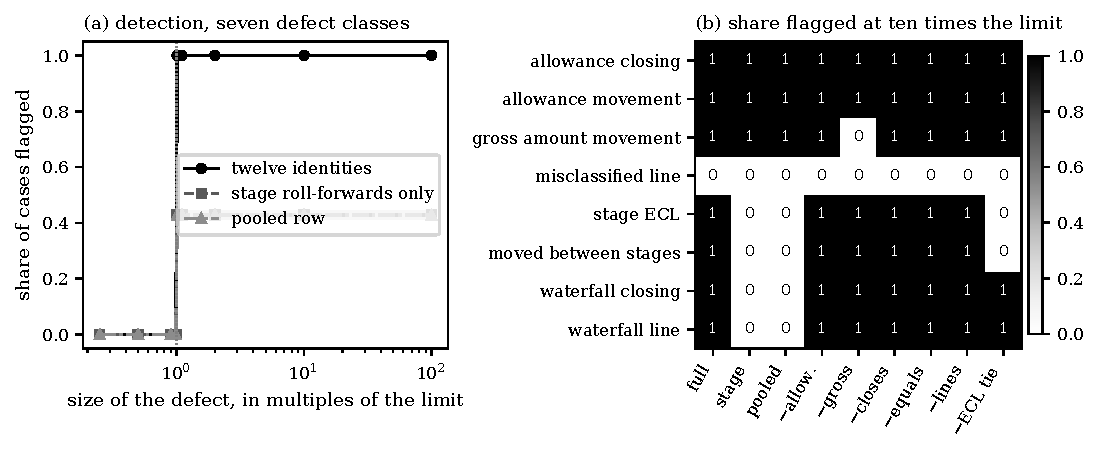
\includegraphics[width=\textwidth]{power}
\caption{Detection of planted defects on the six committed C06 dates. Panel (a) shows the share flagged against the size of the defect in multiples of the limit, pooled over seven defect classes, for the twelve identities, the stage roll-forwards alone and the pooled row, with 95\% Wilson bands. Panel (b) shows the share flagged at ten times the limit, by class and by method, including the full set with one identity family left out.}
\label{fig:power}
\end{figure}

The identities that fail localize the defect to a small group: an allowance movement fails \eoneIdsAllowanceMovement{} identities, an allowance closing \eoneIdsAllowanceClosing{}, a reallocation \eoneIdsStageReallocation{}, a gross-amount movement \eoneIdsGcaMovement{}, a waterfall line \eoneIdsWaterfallLine{}, the waterfall closing \eoneIdsWaterfallClosing{} and a stage ECL \eoneIdsStageEcl{}.
\Cref{fig:incidence} shows the matrix behind this: every entry is seen by at least one equation, the \esixEntries{} entries fall in \esixPatterns{} patterns, and the rank is \esixRank{}.

\begin{figure}[htbp]
\centering
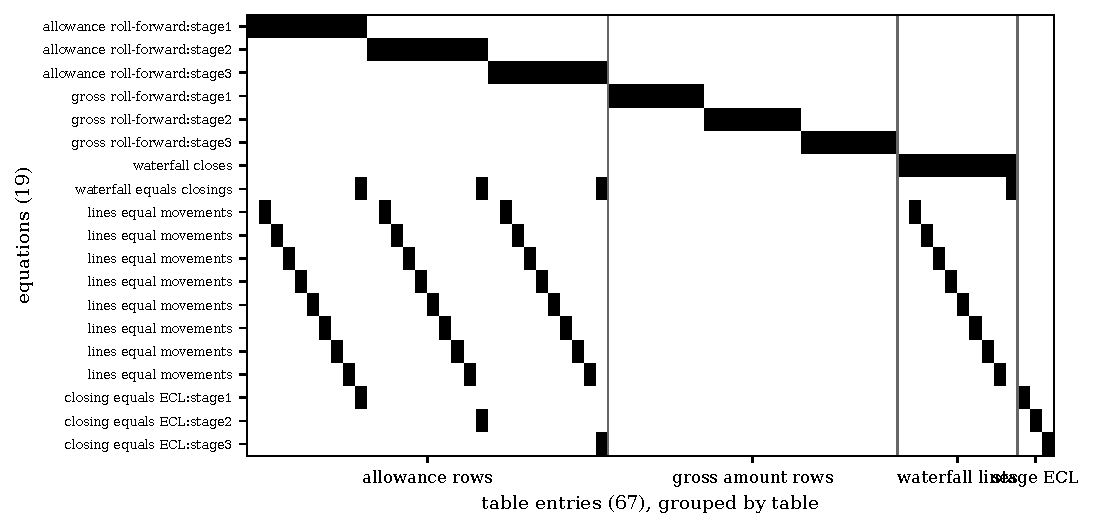
\includegraphics[width=\textwidth]{incidence}
\caption{Absolute value of the signed matrix of the identities for the 2008-12 book: 19 equations in rows and 67 table entries in columns, grouped by table. A dark cell means the entry appears in the equation. Entries with identical columns cannot be told apart by the failing identities.}
\label{fig:incidence}
\end{figure}

\subsection{Tolerance basis and rounding}
\label{sec:res-rounding}

An absolute tolerance of $10^{-6}$ units flags \etwoAbsCommittedK{} of the six clean committed tables and \etwoAbsResK{} of \etwoResN{} resampled books (\etwoAbsResPct{}, Wilson 95\% interval \etwoAbsResLo{} to \etwoAbsResHi{}); absolute tolerances of 0.01 and 1 units, and every relative tolerance from $10^{-12}$ to $10^{-4}$, flag none.
The largest relative residual of a resampled book is \etwoRelMaxResid{}, so the choice of $10^{-6}$ is nine orders above the noise and the tolerance is a policy value, not a numerical necessity.
After rounding every stored number (\cref{tab:rounding}, \cref{fig:rounding}), no book is flagged at units of 1, 10 and 1,000, and \etwoRoundTenThousandK{} of \etwoResN{} at 10,000, as Proposition~\ref{prop:rounding} requires.
At 100,000 units \etwoRoundHundredThousandPct{} are flagged (interval \etwoRoundHundredThousandLo{} to \etwoRoundHundredThousandHi{}), from \etwoHundredLow{} to \etwoHundredHigh{} by date, lower on the larger books whose limit is larger.
At one million units \etwoRoundMillionK{} are flagged (\etwoRoundMillionPct{}, \etwoRoundMillionLo{} to \etwoRoundMillionHi{}); the prediction of more than 99\% was refuted.
The \etwoMillionUnflagged{} books not flagged are spread over the six dates (\etwoMillionUnflaggedDates{}), and the cause is not established.

\begin{figure}[htbp]
\centering
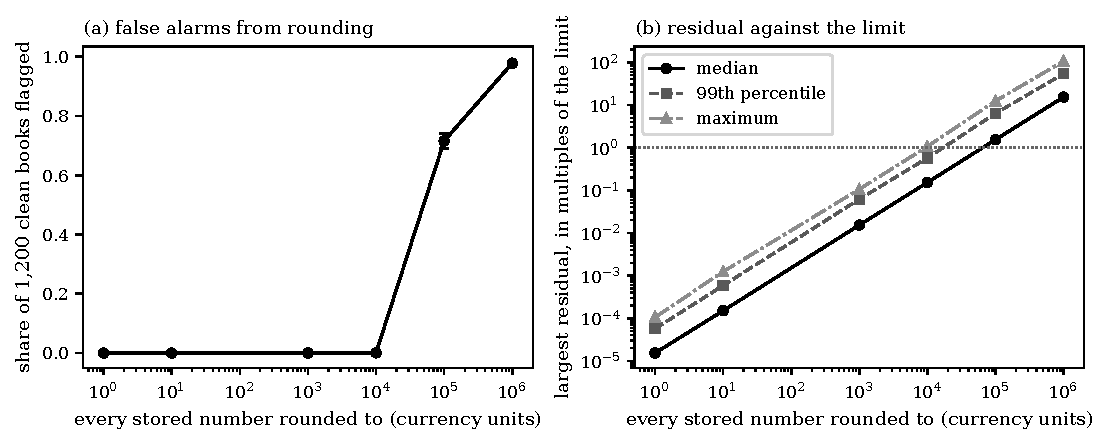
\includegraphics[width=\textwidth]{rounding}
\caption{Rounding of clean resampled books. Panel (a) shows the share of the 1,200 books flagged against the unit to which every stored number is rounded, with Wilson intervals. Panel (b) shows the median, 99th percentile and maximum over books of the largest residual in multiples of the limit; the dotted line at one is the flagging threshold.}
\label{fig:rounding}
\end{figure}

\begin{table}[htbp]
\centering
\small
\caption{False alarms of the test on 1,200 clean resampled books after every stored number is rounded independently to the stated unit: books flagged, and the largest residual of a book as a multiple of the limit (median, 99th percentile and maximum over the books; a value above 1 is a flag).}
\label{tab:rounding}
\begin{adjustbox}{max width=\textwidth}
\begin{tabular}{lrrrrr}
\toprule
Rounded to (units) & Flagged & Percent [Wilson 95\%] & Median & 99th percentile & Maximum \\
\midrule
1 & 0/1,200 & 0.0 [0.0, 0.3] & 0.000 & 0.000 & 0.00 \\
10 & 0/1,200 & 0.0 [0.0, 0.3] & 0.000 & 0.001 & 0.00 \\
1,000 & 0/1,200 & 0.0 [0.0, 0.3] & 0.015 & 0.062 & 0.11 \\
10,000 & 1/1,200 & 0.1 [0.0, 0.5] & 0.152 & 0.572 & 1.06 \\
100,000 & 859/1,200 & 71.6 [69.0, 74.1] & 1.539 & 6.321 & 12.35 \\
1,000,000 & 1,174/1,200 & 97.8 [96.8, 98.5] & 15.255 & 53.850 & 105.91 \\
\bottomrule
\end{tabular}
\end{adjustbox}
\end{table}


\subsection{Overlays}
\label{sec:res-overlays}

In \ethreeSets{} overlay sets drawn at random the model ECL and the ECL by stage never changed and the total was always the model ECL plus the overlays: \ethreeViolations{} violations.
\Cref{tab:placement} gives the placement: the correct booking closes every identity in all \ethreeCases{} cases; the four wrong bookings that put the overlay in some tables and not in others are flagged by the twelve identities in all \ethreeCases{} cases each, by \ethreeIdsNotCarried{}, \ethreeIdsWrongStage{}, \ethreeIdsDoubleCarried{} and \ethreeIdsCarriedNotInWaterfall{} identities, and by neither the stage arithmetic nor the pooled row.
The overlay merged into the model ECL under the remeasurement line closes every identity and is flagged by nothing.
On the synthetic bank the two committed overlays are \ethreeSevenOverlay{} million CLP of an allowance of \ethreeSevenAllowance{} million, \ethreeSevenShare{}, and a merge would overstate the model ECL by \ethreeSevenMerge{}.

\begin{table}[htbp]
\centering
\small
\caption{Six ways to book an overlay of 2\%, 10\% and 25\% of the allowance on each of the six committed dates (18 cases per row): cases flagged by the twelve identities, by the two roll-forwards of each stage alone and by one pooled row, and the number of identities that fail when the booking is flagged.}
\label{tab:placement}
\begin{adjustbox}{max width=\textwidth}
\begin{tabular}{p{6.6cm}rrrr}
\toprule
Booking of an overlay & Twelve identities & Stage arithmetic & Pooled row & Identities failing \\
\midrule
Carried in the stage 1 row, no waterfall line & 18/18 & 0/18 & 0/18 & 3 \\
Correct booking (stage 1 row, waterfall line, both closings) & 0/18 & 0/18 & 0/18 & 0 \\
Carried in stage 1 and stage 2 rows, one waterfall line & 18/18 & 0/18 & 0/18 & 3 \\
Added to the model ECL under the remeasurement line & 0/18 & 0/18 & 0/18 & 0 \\
Waterfall only, stage rows untouched & 18/18 & 0/18 & 0/18 & 3 \\
Carried in the stage 2 row, waterfall line at portfolio level & 18/18 & 0/18 & 0/18 & 2 \\
\bottomrule
\end{tabular}
\end{adjustbox}
\end{table}


\subsection{Non-linearity of the weighted PD}
\label{sec:res-nonlinearity}

Of \efourDraws{} draws, \efourConvexN{} have every factor in the convex region and none has a negative index (smallest \efourConvexMin{}); \efourConcaveN{} have every factor in the concave region and none has a positive index (largest \efourConcaveMax{}); \efourMixedN{} are mixed, with \efourMixedPos{} positive and \efourMixedNeg{} negative indexes, down to \efourMixedMin{} (\cref{fig:sweep}).
The Gauss--Hermite check of the engine is within \efourGhErr{} in every draw.
The second-order formula is within 25\% of the index in \efourSecondWithin{} of \efourSecondN{} convex draws, with a median ratio of \efourSecondQFifty{} and 5th to 95th percentiles of \efourSecondQFive{} to \efourSecondQNinetyFive{}.

\begin{figure}[htbp]
\centering
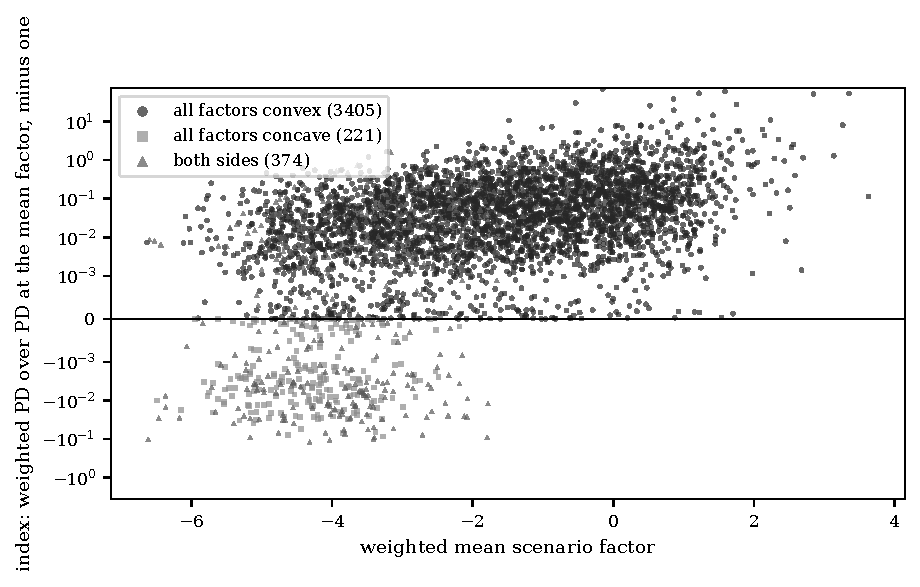
\includegraphics[width=0.85\textwidth]{sweep}
\caption{Index of the weighted PD against the weighted mean scenario factor for the first 4,000 draws of the sweep, by position of the scenario factors relative to the inflection of the conditional PD; the vertical axis is symmetric logarithmic and the horizontal line marks zero.}
\label{fig:sweep}
\end{figure}

On the six committed dates (\cref{tab:committed-nonlinearity}) every scenario lies in the convex region, the inflection is between \efourZstarLow{} and \efourZstarHigh{} and the lowest factor is \efourZminLow{} or higher, the PD-level index runs from \efourPdLow{} to \efourPdHigh{}, and the engine reproduces it to \efourPdAgree{}.
The ECL-level index is positive on \efourEclPositive{} of six dates and \efourEclTen{} on 2010-12, where the Stage 2 share is \efourTenShare{} and the Stage 2 ratio differs by \efourGapTen{} between recomputed and frozen staging, against at most \efourGapOther{} on the other dates.
Staging that responds to the weights is the one feature that distinguishes that date; we did not isolate it as the cause.

\begin{table}[htbp]
\centering
\small
\caption{The six committed C06 dates: the inflection of the conditional PD, the lowest and highest scenario factor, the PD-level index recomputed by the engine from the committed scenario factors (equal to the committed value), the committed ECL-level index, the Stage 2 share of the gross amount and the gap between the Stage 2 ratio under recomputed and frozen staging at the grid weights nearest to the committed ones.}
\label{tab:committed-nonlinearity}
\begin{adjustbox}{max width=\textwidth}
\begin{tabular}{lrrrrrrr}
\toprule
Date & Inflection $z^*$ & Lowest $z$ & Highest $z$ & PD-level index & ECL-level index & Stage 2 share & Stage 2 gap \\
\midrule
2006-12 & -6.41 & -0.99 & -0.81 & 0.00113 & +0.00211 & 0.1\% & 0.00005 \\
2008-12 & -6.16 & -1.48 & -1.35 & 0.00079 & +0.02121 & 1.1\% & 0.00009 \\
2010-12 & -5.73 & -2.46 & -1.61 & 0.01882 & -0.00071 & 56.5\% & 0.01510 \\
2019-12 & -5.74 & -0.01 & 0.50 & 0.01164 & +0.02320 & 0.0\% & 0.00000 \\
2020-06 & -5.75 & -2.15 & -2.07 & 0.00017 & +0.01279 & 96.7\% & 0.00007 \\
2023-06 & -5.82 & 0.03 & 0.30 & 0.00323 & +0.00622 & 0.0\% & 0.00002 \\
\bottomrule
\end{tabular}
\end{adjustbox}
\end{table}


Against the full distribution of the factor (\cref{tab:designs}, \cref{fig:designs}) the base scenario alone has a median absolute error of \efourSingleMed{} (\efourSingleMedLo{} to \efourSingleMedHi{}), three scenarios at one standard deviation \efourAdhocMed{}, tertile means \efourTertileMed{}, the three-point rule \efourGhThreeMed{} and the five-point rule \efourGhFiveMed{}.
Among the \efourStrong{} draws with a margin of two standard deviations inside the convex region, the base scenario and the 25/50/25 set understate the expected PD in \efourSingleUnder{} and \efourAdhocUnder{}; the median ratio of the predicted to the measured bias of the 25/50/25 set is \efourBiasMedian{}.

\begin{figure}[htbp]
\centering
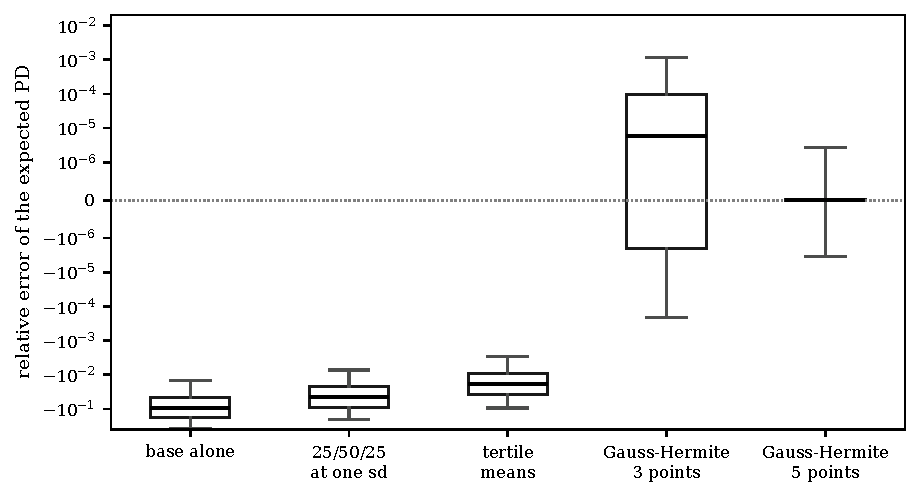
\includegraphics[width=0.85\textwidth]{designs}
\caption{Relative error of the expected PD for five scenario sets against the 64-node Gauss--Hermite expectation, over 5,000 draws: boxes span the quartiles, whiskers the 5th and 95th percentiles, the thick line is the median; the axis is symmetric logarithmic.}
\label{fig:designs}
\end{figure}

\begin{table}[htbp]
\centering
\small
\caption{Relative error of the expected PD of five scenario sets against the 64-node Gauss--Hermite expectation under a normal factor, over 5,000 draws of the PD, the correlation and the forecast mean and spread: quantiles of the signed error in percent, the share of draws with absolute error above 5\%, and the share understated among the draws whose forecast lies two standard deviations inside the convex region.}
\label{tab:designs}
\begin{adjustbox}{max width=\textwidth}
\begin{tabular}{p{5.2cm}rrrrr}
\toprule
Scenario set & 5th pct (\%) & Median (\%) & 95th pct (\%) & $|$error$|>5\%$ & Understated (convex margin) \\
\midrule
Base scenario alone & -38 & -9.2 & -1.47 & 72.4\% & 100.0\% \\
Three scenarios at one standard deviation, 25/50/25 & -19.9 & -4.56 & -0.727 & 46.4\% & 100.0\% \\
Three equal-probability tertile means & -9.4 & -1.84 & -0.293 & 16.7\% & 100.0\% \\
Three-point Gauss--Hermite & -0.0211 & +0.0006 & +0.119 & 0.0\% & 29.2\% \\
Five-point Gauss--Hermite & -0.000336 & +4.27e-09 & +0.000267 & 0.0\% & 41.1\% \\
\bottomrule
\end{tabular}
\end{adjustbox}
\end{table}


\subsection{Three regimes on one synthetic bank}
\label{sec:res-regimes}

\Cref{tab:regimes} and \cref{fig:regimes} give the committed totals and the ten-seed ratios.
The committed base scenario has B-1 \efiveCommittedBaseB{}, IFRS 9 \efiveCommittedBaseI{} and Annex 9 \efiveCommittedBaseA{} billion CLP; the combined severe scenario \efiveCommittedCombinedB{}, \efiveCommittedCombinedI{} and \efiveCommittedCombinedA{}.
The committed seed is reproduced to \efiveCommittedDiff{} currency units.
Over \efiveSeeds{} seeds the IFRS 9 over B-1 ratio is \efiveBaseMean{} in the base (95\% interval \efiveBaseLo{} to \efiveBaseHi{}, standard deviation \efiveBaseSd{}) and \efiveCombinedMean{} in the combined severe scenario (\efiveCombinedLo{} to \efiveCombinedHi{}); it is below one in the other five scenarios and above one in the severe one \efiveOrder{}.
IFRS 9 exceeds Annex 9 in the base in \efiveIfrsAboveBde{} seeds of \efiveSeeds{}.
The bridge closes within \efiveBridgeMax{} units in all \efiveCells{} runs and the engine's reconciliation test is green in \efiveGreen{} of them.
In the base the mean steps are $\efiveStepBaseMeasurementBasis$ billion for the measurement basis, $+\efiveStepBaseLifetimeHorizon$ for the lifetime horizon, $+\efiveStepBaseForwardLooking$ for probability weighting, $+\efiveStepBaseDiscounting$ for discounting and $+\efiveStepBaseIfrsNineOverlays$ for overlays; the B-1 minimum is not binding.
The non-linearity index of the IFRS 9 allowance averages \efiveNlBase{} (\efiveNlBaseLow{} to \efiveNlBaseHigh{}) in the base.

\begin{figure}[htbp]
\centering
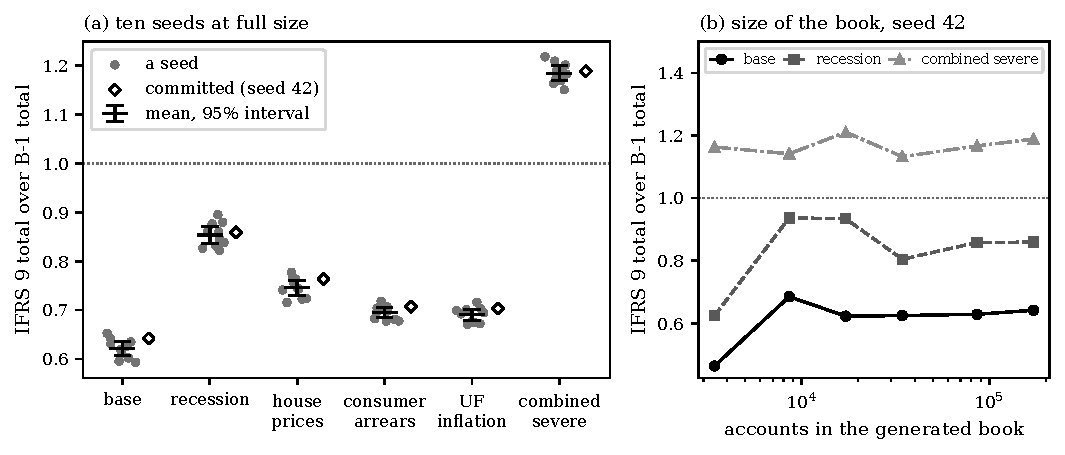
\includegraphics[width=\textwidth]{regimes}
\caption{IFRS 9 total over B-1 total of the synthetic bank. Panel (a) shows, for each scenario, the ten seeds at full size (grey dots), their mean with a 95\% interval and the committed seed 42 (diamond). Panel (b) shows seed 42 at six sizes of the generated book; the dotted line at one marks equal totals.}
\label{fig:regimes}
\end{figure}

\begin{table}[htbp]
\centering
\small
\caption{The three provisioning regimes on the synthetic Banco Andino in six scenarios: the committed totals (seed 42, full size), their ratio, and the mean over ten seeds at full size of the IFRS 9 and Annex 9 totals over the B-1 total with the 95\% $t$ interval of the mean in brackets.}
\label{tab:regimes}
\begin{adjustbox}{max width=\textwidth}
\begin{tabular}{lrrrrrr}
\toprule
Scenario & B-1 (CLP bn) & IFRS 9 (CLP bn) & Annex 9 (CLP bn) & IFRS 9/B-1 & IFRS 9/B-1, ten seeds & Annex 9/B-1, ten seeds \\
\midrule
Base & 152.0 & 97.6 & 79.6 & 0.642 & 0.621 [0.606, 0.635] & 0.549 [0.532, 0.566] \\
Recession & 197.5 & 169.8 & 116.3 & 0.860 & 0.854 [0.836, 0.871] & 0.601 [0.584, 0.618] \\
House price fall & 168.9 & 128.8 & 94.6 & 0.763 & 0.746 [0.731, 0.760] & 0.599 [0.581, 0.617] \\
Consumer arrears shock & 178.6 & 126.3 & 97.3 & 0.707 & 0.694 [0.684, 0.705] & 0.581 [0.566, 0.596] \\
UF inflation spike & 166.9 & 117.4 & 85.6 & 0.703 & 0.690 [0.679, 0.701] & 0.552 [0.536, 0.568] \\
Combined severe & 275.8 & 327.8 & 191.6 & 1.189 & 1.185 [1.170, 1.200] & 0.699 [0.679, 0.719] \\
\bottomrule
\end{tabular}
\end{adjustbox}
\end{table}


The ratios depend on the size of the book (\cref{tab:ladder}): at \efiveLadderLowAccounts{} accounts the base ratio is \efiveLadderLowBase{} against \efiveLadderHighBase{} at full size, while the combined severe ratio is above one at \efiveLadderSevereAbove{} of \efiveLadderCount{} sizes.

\begin{table}[htbp]
\centering
\small
\caption{The IFRS 9 total over the B-1 total of the synthetic bank at seed 42 for six sizes of the generated book (the size factor scales every portfolio's account count), with the largest bridge residual over the six scenarios in currency units and the measured time of one build of the six scenarios.}
\label{tab:ladder}
\begin{adjustbox}{max width=\textwidth}
\begin{tabular}{rrrrrrr}
\toprule
Size factor & Accounts & Base & Recession & Combined severe & Bridge residual & Seconds \\
\midrule
0.02 & 3,430 & 0.464 & 0.625 & 1.163 & 2.4e-07 & 4 \\
0.05 & 8,575 & 0.685 & 0.937 & 1.142 & 7.2e-07 & 5 \\
0.1 & 17,150 & 0.623 & 0.934 & 1.211 & 3.8e-06 & 16 \\
0.2 & 34,300 & 0.625 & 0.805 & 1.133 & 3.8e-06 & 37 \\
0.5 & 85,750 & 0.629 & 0.858 & 1.167 & 2.3e-05 & 86 \\
1 & 171,500 & 0.642 & 0.860 & 1.189 & 3.1e-05 & 56 \\
\bottomrule
\end{tabular}
\end{adjustbox}
\end{table}


\subsection{Outcome of the predictions}
\label{sec:res-hypotheses}

\hypHeld{} of \hypTotal{} predictions held and \hypRefuted{} were refuted: \hypRefutedList{}.
The rounding to millions (Q3b), the one blind entry (A2) and the group of eleven entries (A4) were wrong in their numbers; the weighted ECL above the mean path on every committed date (S3) is contradicted by 2010-12.

\begin{table}[htbp]
\centering
\small
\caption{Main comparison of the proposed protocol with the comparators run on the same data: detection of planted defects by the twelve identities, the stage arithmetic and the pooled row; false alarms on clean tables by tolerance basis; overlay bookings; the non-linearity of the weighted PD; the error of short scenario sets against the full distribution of the factor; and the three regimes of the synthetic bank over ten seeds. Intervals as stated in the last column.}
\label{tab:main-results}
\begin{adjustbox}{max width=\textwidth}
\begin{tabular}{p{5.4cm}p{3.3cm}p{4.0cm}p{3.0cm}}
\toprule
Measurement & Proposed protocol & Comparator & Uncertainty \\
\midrule
Detection above the limit (1.01 times), seven defect classes, 600 cases each & 4,200/4,200 [99.9, 100.0] & stage 1,800/4,200 [41.4, 44.4]; pooled 1,800/4,200 [41.4, 44.4] & Wilson 95\% interval, percent \\
Detection below the limit (0.99 times), eight classes & 0/4,800 [0.0, 0.1] & stage 0/4,800; pooled 0/4,800 & Wilson 95\% interval, percent \\
Smallest defect named, as a multiple of the limit, 120 bisections per class & 1 within $2.4\times10^{-10}$ & not applicable (no comparator names a size) & largest deviation over 840 bisections \\
Clean committed tables flagged (six dates) & 0/6 (relative 1e-6) & 4/6 (absolute 1e-6) & count, no sampling \\
Clean resampled books flagged (1,200) & 0/1,200 [0.0, 0.3] & absolute 1e-6: 68/1,200 [4.5, 7.1] & Wilson 95\% interval, percent \\
Wrong overlay bookings detected (four kinds, 18 cases each) & 72/72 & stage 0/72; pooled 0/72 & count over the full enumeration \\
Negative index among draws in the convex region & 0/16,906 & unqualified statement fails in 1,844/20,000 draws & count over the sweep \\
Median absolute error of the expected PD, base scenario alone & not applicable & 9.20\% [8.94, 9.54] & bootstrap 95\% interval \\
Median absolute error, three scenarios at one standard deviation, 25/50/25 & not applicable & 4.56\% [4.41, 4.75] & bootstrap 95\% interval \\
Median absolute error, three equal-probability tertile scenarios & not applicable & 1.84\% [1.77, 1.92] & bootstrap 95\% interval \\
Median absolute error, three-point Gauss--Hermite scenarios & not applicable & $3.0\times10^{-3}$\% [$2.7\times10^{-3}$, $3.4\times10^{-3}$] & bootstrap 95\% interval \\
IFRS 9 over B-1, base scenario, ten seeds & 0.621 [0.606, 0.635] & B-1 is the reference (1) & mean and 95\% $t$ interval \\
IFRS 9 over B-1, combined severe scenario, ten seeds & 1.185 [1.170, 1.200] & B-1 is the reference (1) & mean and 95\% $t$ interval \\
Largest bridge residual, 60 runs (currency units) & $3.8\times10^{-5}$ & not applicable & maximum, no sampling \\
\bottomrule
\end{tabular}
\end{adjustbox}
\end{table}

\begin{longtable}{lp{7.6cm}p{4.4cm}}
\caption{The 31 statements tested by the experiments, each stated in the header of its script, with what the header and the history of the design document say about when it was set; the repository does not record whether a prediction preceded the first run of its script. The 27 statements whose result no committed document held are predictions; the 4 others (B6, C1, C2, C3) are reproductions and are not counted as predictions.}\label{tab:hypotheses}\\
\toprule
ID & Statement & Set \\
\midrule
\endfirsthead
\toprule
ID & Statement & Set \\
\midrule
\endhead
\bottomrule
\endfoot
P1 & The smallest defect the test names equals the limit for every class but the misclassification. & stated in the script header; the notebook had measured it on one defect class \\
P2 & The pooled row and the stage arithmetic detect three classes above the limit and none of the other four; the twelve identities detect all seven. & stated in the script header \\
P3 & Leaving out one identity family loses a class entirely for exactly two families: the gross amount roll-forward and the tie to the ECL. & stated in the script header \\
Q1 & An absolute tolerance of 1e-6 units flags a clean committed table; the relative basis flags none of the six or of the 1,200 resampled books. & stated in the script header; the notebook had measured the flag on a committed table \\
Q2 & After rounding to 1, 10 and 1,000 units no book is flagged; at 10,000 fewer than 1\% are. & stated in the script header \\
Q3a & After rounding to 100,000 units between 30\% and 95\% of the books are flagged. & stated in the script header \\
Q3b & After rounding to 1,000,000 units more than 99\% of the books are flagged. & stated in the script header \\
O1 & The model ECL does not depend on the overlays and the total is the model ECL plus the overlays, in 3,000 draws. & stated in the script header \\
O2 & The correct overlay booking closes every identity in 18 of 18 cases. & stated in the script header \\
O3 & The twelve identities flag four wrong overlay bookings in 18 of 18 cases each; the stage arithmetic and the pooled row flag none. & stated in the script header \\
O4 & No method flags an overlay merged into the model ECL. & stated in the script header \\
N1 & No negative index among the draws whose factors all lie in the convex region. & stated in the script header; the notebook had swept another seed \\
N2 & No positive index among the draws whose factors all lie in the concave region, with at least 100 such draws. & stated in the script header \\
N3 & Both signs occur among the draws with factors on both sides of the inflection. & stated in the script header \\
N4 & The second-order formula is within 25\% of the index in at least 75\% of the convex draws. & stated in the script header \\
R1 & Where the forecast lies two standard deviations inside the convex region the base scenario alone understates the expected PD in at least 99\% of the draws. & stated in the script header \\
R2 & The median absolute error is ordered gh5 < gh3 < tertile3 < adhoc3 < single. & stated in the script header \\
R3 & The second-order bias of the three-scenario set is within 20\% of the measured bias at the median. & stated in the script header \\
B1 & The bridge closes to within one currency unit in every seed and scenario. & stated in the script header \\
B2 & The engine's reconciliation test is green in every seed and scenario. & stated in the script header \\
B3 & IFRS 9 is below B-1 in five scenarios and above it in the combined severe scenario, in every seed. & stated in the script header \\
B4 & IFRS 9 is above Annex 9 in the base scenario in at least 8 of 10 seeds. & stated in the script header \\
B5 & The standard deviation over seeds of the base IFRS 9 over B-1 ratio is below 0.05. & stated in the script header \\
B6 & The committed seed at the committed size reproduces every committed regime total to within one currency unit (reproduction of the committed totals). & after the bake; the committed totals had been read \\
A1 & The engine's residuals equal the signed map times the perturbation for every entry of the six dates. & stated in the script header \\
A2 & Exactly one entry is seen by no identity: the model ECL of the POCI stage. & stated in the script header \\
A3 & The signed map has full row rank. & stated in the script header \\
A4 & The largest group of entries no failing pattern distinguishes has at least 11 entries. & stated in the script header \\
C1 & The reference example gives a weighted PD of 2.68\% against 1.80\% at the mean factor (reproduction of the acceptance criterion). & before the bake (design document, 5 October 2026); the bake was built to meet it \\
C2 & The identities close on the tolerance basis on the six committed dates (reproduction of the acceptance criterion). & before the bake (design document, 5 October 2026); the bake was built to meet it \\
C3 & The weighted ECL exceeds the ECL at the mean path on every committed date (stated in the product as not claimed). & after the bake; stated in the product as not claimed \\
\end{longtable}

\begin{table}[htbp]
\centering
\small
\caption{The six committed reporting dates of the SBA 7(a) loan book: the gross carrying amount G, the limit of the test on the engine's tolerance basis, the share of the gross amount in Stage 2, the number of loans in the staged book and the largest residual of the twelve identities on the committed tables.}
\label{tab:data}
\begin{adjustbox}{max width=\textwidth}
\begin{tabular}{lrrrrr}
\toprule
Date & Gross amount G (USD bn) & Limit $10^{-6}G$ (USD) & Stage 2 share & Loans & Largest residual (USD) \\
\midrule
2006-12 & 47.1 & 47,124 & 0.1\% & 305,319 & $1.5\times10^{-5}$ \\
2008-12 & 47.2 & 47,248 & 1.1\% & 311,503 & $1.2\times10^{-7}$ \\
2010-12 & 55.5 & 55,460 & 56.5\% & 280,265 & $3.8\times10^{-6}$ \\
2019-12 & 99.6 & 99,603 & 0.0\% & 271,801 & $1.5\times10^{-5}$ \\
2020-06 & 99.7 & 99,711 & 96.7\% & 268,493 & $1.3\times10^{-5}$ \\
2023-06 & 116.8 & 116,761 & 0.0\% & 251,636 & $1.2\times10^{-7}$ \\
\bottomrule
\end{tabular}
\end{adjustbox}
\end{table}


\section{Ablation}
\label{sec:ablation}

The protocol has components whose contribution can be removed one at a time: the identity families, the relative tolerance, the separate overlay line, the region qualifier of the non-linearity statement and the weighting of scenarios.
Each removal is measured on the experiment that exercises the component.

\subsection{Identity families}
\label{sec:ablation-families}

\Cref{tab:ablation} leaves out one of the six identity families and reports the share of the \eoneCases{} cases of each defect class, planted at ten times the limit, that the remaining identities still flag.
Exactly \eoneFamiliesLost{} families are irreplaceable for detection: the gross-amount roll-forward, without which a gross-amount movement is never flagged, and the tie of the stage closing to the stage ECL and the overlays, without which a reallocation between stages and a change of the stage ECL are never flagged.
The other four families, the allowance roll-forward and the three waterfall identities, are redundant for single-entry detection, because every class they see is also seen by another family; they remain useful for localization, since they change the number of failing identities from one or two to the values of Section~\ref{sec:res-detection}.
The comparator that keeps only the two roll-forwards of each stage is the removal of the four cross families at once, and it loses four classes.
This is the prediction P3, which held.

\begin{table}[htbp]
\centering
\small
\caption{Ablation of the twelve identities by family: share of the 600 cases of each defect class (defect of ten times the limit) that the remaining identities still flag when one family is left out; the last column counts the classes that no remaining identity detects.}
\label{tab:ablation}
\begin{adjustbox}{max width=\textwidth}
\begin{tabular}{p{4.6cm}rrrrrrrr}
\toprule
Identity family left out & Alw. mov. & Alw. clos. & Realloc. & GCA mov. & WF line & WF clos. & Stage ECL & Classes lost \\
\midrule
Allowance roll-forward by stage & all & all & all & all & all & all & all & 0 \\
Gross amount roll-forward by stage & all & all & all & 0 & all & all & all & 1 \\
Waterfall closes & all & all & all & all & all & all & all & 0 \\
Waterfall equals stage closings & all & all & all & all & all & all & all & 0 \\
Waterfall lines equal stage movements & all & all & all & all & all & all & all & 0 \\
Stage closing equals ECL plus overlays & all & all & 0 & all & all & all & 0 & 2 \\
None left out (twelve identities) & all & all & all & all & all & all & all & 0 \\
\bottomrule
\end{tabular}
\end{adjustbox}
\end{table}


\subsection{The other components}
\label{sec:ablation-components}

\Cref{tab:ablation-components} measures the other components.
Replacing the relative tolerance by an absolute tolerance of $10^{-6}$ units moves the false alarms on clean resampled books from none to \etwoAbsResPct{}.
Removing the cross identities lowers the detection above the limit from \eoneAboveFullK{} of \eoneAboveFullN{} to \eoneAboveStageK{}.
Replacing the separate overlay line by a merge leaves nothing to test: every table closes and the model ECL is overstated by the overlay share over one minus the share.
Dropping the region qualifier makes the statement that the weighted PD is at least the PD at the mean factor false in \efourConcaveNeg{} concave draws and \efourMixedNeg{} mixed draws, against none of the \efourConvexN{} convex draws.
Replacing weighted scenarios by the base scenario alone raises the median absolute error of the expected PD from \efourGhThreeMed{} for the three-point rule to \efourSingleMed{}.

\begin{table}[htbp]
\centering
\small
\caption{Ablation of the other components of the protocol, each measured on the experiment that exercises it: the tolerance basis, the cross identities, the separate overlay line, the region qualifier of the non-linearity statement and the weighting of scenarios, with the value of the measure with and without the component.}
\label{tab:ablation-components}
\begin{adjustbox}{max width=\textwidth}
\begin{tabular}{p{4.8cm}p{3.6cm}p{3.4cm}p{3.4cm}}
\toprule
Component removed & Measure & With the component & Without it \\
\midrule
Relative tolerance basis replaced by an absolute tolerance of 1e-6 units & false alarms on clean books & 0/1,200 [0.0, 0.3] & 68/1,200 [4.5, 7.1] \\
Cross identities removed (stage arithmetic only) & detection above the limit, seven classes & 4,200/4,200 [99.9, 100.0] & 1,800/4,200 [41.4, 44.4] \\
Separate overlay line replaced by a merge into the model ECL & wrong bookings of the overlay detected & 72/72 (four kinds) & not applicable: no line to test \\
Convex-region qualifier dropped from the non-linearity statement & draws that contradict the statement & 0/16,906 (qualified) & 1,844/20,000 (unqualified) \\
Probability-weighted scenarios replaced by the base scenario alone & median absolute error of the expected PD & 0.0030\% (three-point) & 9.20\% \\
\bottomrule
\end{tabular}
\end{adjustbox}
\end{table}


\section{Discussion}
\label{sec:discussion}

\subsection{What the limits mean for a validator}
\label{sec:disc-limits}

A green reconciliation is a statement with a size.
On the books studied it says that no entry is wrong by more than about forty-seven to one hundred and seventeen thousand USD, which is one millionth of the gross carrying amount, and nothing about defects that leave every sum unchanged.
The size is a property of the tolerance and of the book, and the tolerance is a choice: because the noise of the sums is about nine orders below it, the limit could be tightened by several orders for tables kept at full precision, and has to be loosened for tables published in rounded units.
For a unit $u$ the guarantee of Proposition~\ref{prop:rounding} needs $\tol\ge qu/(2\gross)$; a validator who receives tables in millions should reconcile with a tolerance of the order of $10^{-4}$ and state the limit that results, or ask for the unrounded tables.
The experiment shows why the choice matters in both directions: an absolute tolerance flags clean books for a reason that has nothing to do with the books, and a tolerance blind to rounding flags nearly all books disclosed in millions.

The cross identities matter more than their number suggests.
The stage arithmetic of the disclosure cannot see a waterfall that disagrees with the tables, a stage ECL that disagrees with the closing, or an allowance moved between stages with both rows closing; the last is the defect that changes staging-dependent disclosures while leaving the total unchanged.
A stage-level check cannot see them.

\subsection{Why the blind spots are structural}
\label{sec:disc-blind}

The two defects that no identity sees, a misclassification between lines and an overlay merged into the model loss, are both in the kernel of the matrix of the identities.
They cannot be removed by adding identities among the same entries; they need information that is not in the tables, such as the registry of approved overlays against which the overlay lines are compared, or an independent recomputation of the model ECL.
The merge is the more consequential, because it is the practice the separate-line rule exists to prevent and because its size can be large: a quarter of the allowance in overlays overstates the model ECL by a third.
The protocol's answer is contractual, not arithmetic: the engine offers an overlay line as the only way to add an amount that is not model ECL, the invariance sweep shows that the engine honours it, and the placement test shows that a line booked in some tables and not others is refused.

\subsection{The non-linearity statement and the committed date}
\label{sec:disc-nonlinearity}

The statement that the weighted PD is at least the PD at the mean factor holds as a theorem in the convex region and fails in the concave region, so it is a statement with a region.
In \efourDraws{} draws the unqualified statement is contradicted in \efourConcaveNeg{} concave and \efourMixedNeg{} mixed cases, about nine per cent of the sweep.
All six committed dates lie in the convex region of the PD-level statement, so the PD-level index is positive there.
The ECL-level index is a different quantity, to which Proposition~\ref{prop:convexity} does not apply, so a negative value on one date does not contradict it.
Of the six dates, 2010-12 has the staging that responds most to the weights (Stage 2 gap \efourGapTen{} against at most \efourGapOther{} elsewhere), but whether that causes the negative value is not established.

The error of a short scenario set is large relative to the effects discussed in practice.
Three scenarios at one standard deviation with weights 25/50/25 understate the expected PD by a median of \efourAdhocMed{}, nearly half of the draws by more than five per cent, because they carry half the variance of the factor; the formula of Proposition~\ref{prop:bias} gives a median ratio of predicted to measured bias of \efourBiasMedian{}.
A moment-matched set costs the same three scenarios and brings the error to the order of $10^{-5}$ in relative terms.
That result is about the PD level with a normal factor; the allowance involves staging, discounting and loss given default, and the transfer of the conclusion to them is not tested.

\subsection{Three regimes on one book}
\label{sec:disc-regimes}

The ordering of the regimes on the synthetic bank is stable across seeds: IFRS 9 below B-1 in five scenarios and above it in the combined severe scenario, and above Annex 9 in the base.
The bridge shows where the gap comes from: in the base most of it is the measurement basis, the first step, which compares the bank's own PD, LGD and recoveries with the statutory matrices, and the model ECL then rises with the lifetime horizon, the weighting and the discounting; the discounting raises it because it lowers the stage 1 and 2 losses and raises the stage 3 loss, the exposure minus the discounted recoveries, by more.
Proposition~\ref{prop:bridge} limits what the closure proves.
The ratios depend on the size of the generated book, possibly because the generator's calibration to the published aggregates has minimum counts, an effect not isolated at the smallest size, so the committed ratios are not size-free and the six sizes should be read as a sensitivity, not a convergence.
The comparison is between three texts applied to one synthetic book; it says nothing about which text is right or about any bank.

\section{Limitations}
\label{sec:limitations}

\subsection{Internal validity}
\label{sec:lim-internal}

The defects are planted by the author's own functions, in eight classes chosen to exercise the identities, and the detection results are properties of those classes.
A defect class not in the list may behave differently, and the first proposition states the general case only for single-entry defects.
Several results are structural: the limit equal to the tolerance follows from linearity, the comparators' blindness to four classes follows from the span of the identities they use, and the overlay placement results follow from which tables each booking touches.
The experiments confirm that the engine implements the structure, entry by entry, and that is their contribution; they are not empirical discoveries about banks.
The resampled books close exactly by construction, so false alarms measured on them isolate floating-point noise and rounding, not the errors of a real preparation process.
The predictions were stated in the script headers by the author of the experiments, which is not independent of the author of the protocol, and the scripts and their outputs entered the repository in one change, so the repository does not record whether a prediction preceded the first run of its script.
The wording of the refuted predictions (the share after rounding to millions, the number of blind entries, the largest group) records numbers the author got wrong.

\subsection{External validity}
\label{sec:lim-external}

The six dates come from one loan book, the SBA 7(a) program, which holds small-business loans with real outcomes but has no POCI row, no overlays and a staging that depends on one model; the overlays of the placement experiment are constructed.
The synthetic bank is calibrated to public aggregates of the CMF and is not a real bank; its totals under the three regimes are a property of the generator and the engine's transcription of the regimes.
The sweeps use the one-factor Gaussian conditional PD; other link functions have other inflection points, and a logistic hazard is convex only where the hazard is below one half.
The scenario-set comparison is at the PD level with a normal factor, not at the allowance level.
The product's staging uses one set of thresholds, and other staging policies would change the Stage 2 share and with it the ECL-level comparisons.
The convex-region theorem does not apply to the ECL-level index of the committed documents, and the reason the 2010-12 index is negative is not established here.

\subsection{Construct validity and scope}
\label{sec:lim-construct}

The identities are necessary conditions for a correct allowance.
A book that reconciles can be wrong in every entry by the same compensating amounts, and the protocol makes no claim that any figure is compliant with a regulation or that any regime is right.
The tolerance of $10^{-6}$ is the engine's internal choice, not a regulatory threshold, and the paper shows its consequences rather than justifying it.
The bridge closes by construction up to the agreement of two aggregations, as Proposition~\ref{prop:bridge} states, so its closure is not a validation of the size of any step.
The search for a public comparison of the three regimes on one portfolio was bounded by the sources named in Section~\ref{sec:related-work}, and the absence of such a comparison is not established beyond them.
The detection limit is stated in units of the book; a book in another currency or scale has another limit with the same ratio to its gross carrying amount.
The prediction of the first experiment about the reproduction of a notebook measurement is of the same kind as the others and is not evidence of independence from it.

\section{Reproducibility}
\label{sec:reproducibility}

The source, the committed documents and the scripts are in the repository named in the header of the paper.
The engine is \texttt{riskvalidation} 1.1.0 from the Python Package Index, and the C06 and C07 documents were baked on it.
Each experiment is one script run from the repository root with the product's interpreter, \texttt{python manuscripts/provisions-reconciliation-identities/experiments/e1\_gate\_power.py} and likewise for the scripts \texttt{e2} to \texttt{e6}; the fifth is run with a list of seeds and a list of sizes, once for the ten seeds at full size, \texttt{e5\_regimes.py --seeds 42 1 2 3 4 5 6 7 8 9 --scale 1.0}, and once for seed 42 at six sizes, \texttt{e5\_regimes.py --seeds 42 --scale 0.02 0.05 0.1 0.2 0.5}, with the committed size taken from the first.
Each writes compact JSON next to itself with sorted keys, and a rerun with the same seeds gives the same bytes; the seed of every draw is derived from a base seed and the indices of the experiment.
The measured run times are \eoneSeconds{} seconds for the first, \etwoSeconds{} seconds for the second, \ethreeSeconds{} seconds for the third, \efourSeconds{} seconds for the fourth (on a workstation running other jobs) and \efiveSecLow{} to \efiveSecHigh{} seconds for one build of the six scenarios at full size; the sixth script does not time itself.
The numbers quoted in the text are macros written by \texttt{make\_numbers.py}, the tables by \texttt{make\_tables.py} and the vector figures by \texttt{make\_figures.py}, all from the experiment outputs; the references are written by \texttt{fetch\_references.py} from the publishers' records. The date at which each reproduced criterion entered the design document is read once from the history of the repository by \texttt{experiments/sdd\_dates.py} and stored in \texttt{experiments/sdd\_dates.json}, which the table script reads, so the tables rebuild without that history.
The datasets are the six committed C06 documents and the six committed C07 documents with the models document; the raw SBA files are public and are read only by the C06 bake.

\section{Conclusions}
\label{sec:conclusions}

The reconciliation identities of an expected credit loss allowance can be run as an acceptance test whose detection limit is known in the units of the book: with twelve identities on a tolerance of one millionth of the gross carrying amount, every planted defect of seven classes is named from the limit, \eoneAboveFullK{} of \eoneAboveFullN{} cases, where the stage arithmetic and a pooled row name \eoneAboveStageK{}.
The test cannot see an amount booked under another line or an overlay merged into the model loss, and it is compatible with tables disclosed in thousands but not in millions; an absolute tolerance flags clean books.
Overlays kept as separate lines leave the model estimate unchanged in \ethreeSets{} random sets, and the identities refuse four wrong bookings of an overlay.
The weighted PD is not below the PD at the mean factor when every scenario lies in the convex region, and a three-scenario set at one standard deviation understates the expected PD by a median of \efourAdhocMed{}.
One synthetic bank has an IFRS 9 total of \efiveBaseMean{} of the B-1 total in the base and above it in the combined severe scenario, in every seed, with a bridge that closes by construction up to the agreement of two aggregations.
The next steps are tests of the overlay registry and of an independent recomputation of the model ECL, which are the information the tables lack, and the extension of the scenario-set comparison from the PD level to the allowance.


\bibliographystyle{plainnat}
\bibliography{references}

\end{document}
